\chapter{El grupo fundamental}

\section{Homotopía por arcos}

\begin{definicion}
    Sean $X$ e $Y$ dos espacios topologicos y $f,g:X\to Y$ dos aplicaciones continuas. Decimos que $f$ es \textbf{homotópica} a $g$ si existe $H:X\times[0,1]\to Y$ continua tal que 
    \begin{gather*}
        H(x,0) = f(x) \hspace{0.5cm} \text{ y } \hspace{0.5cm} H(x,1) = g(x) \ \ \ \forall x\in X
    \end{gather*}

    \begin{figure}[H]
        \centering
        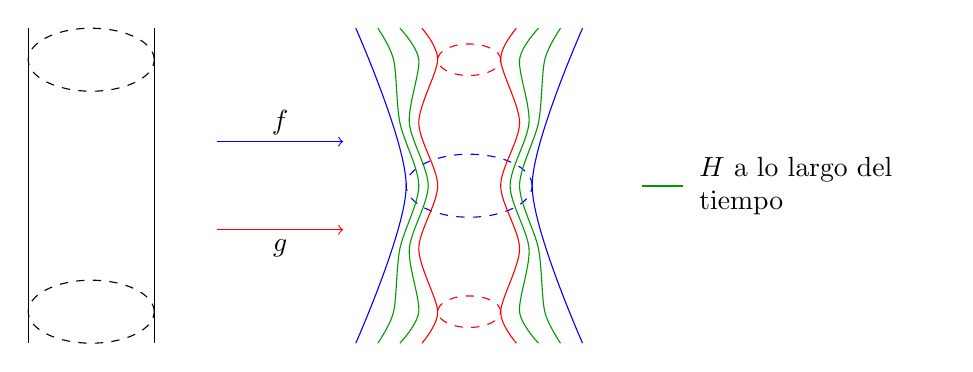
\begin{tikzpicture}[scale=0.8]
            \shorthandoff{>}

            % Cilindro 
            \draw[dashed] (-3,2) ellipse (1 and 0.5);
            \draw[dashed] (-3,-2) ellipse (1 and 0.5);
            \draw (-4,-2.5) -- (-4,2.5);
            \draw (-2,-2.5) -- (-2,2.5);

            % Flecha f
            \node at (0,1) {$f$};
            \draw[->, blue] (-1,0.7) -- (1,0.7);

            % Flecha g
            \node at (0,-1) {$g$};
            \draw[->, red] (-1,-0.7) -- (1,-0.7);

            % Leyenda H
            \node[text width=3cm, anchor=west] at (6.5,0) {$H$ a lo largo del tiempo};
            \draw[thick, green!60!black] (5.75,0)--(6.4,0);

            % Imagen de f
            \draw[dashed, blue] (3,0) ellipse (1 and 0.5);
            \draw[blue] plot[smooth] coordinates {
                (1.2,-2.5) (2,0) (1.2,2.5)
            };
            \draw[blue] plot[smooth] coordinates {
                (4.8,-2.5) (4,0) (4.8,2.5)
            };

            % Imagen de g
            \draw[dashed, red] (3,2) ellipse (0.5 and 0.25);
            \draw[dashed, red] (3,-2) ellipse (0.5 and 0.25);
            \draw[red] plot[smooth] coordinates {
                (2.25,2.5) (2.5,2) (2.2,1) (2.5,0) (2.2,-1) (2.5,-2) (2.25,-2.5)
            };
            \draw[red] plot[smooth] coordinates {
                (3.75,2.5) (3.5,2) (3.8,1) (3.5,0) (3.8,-1) (3.5,-2) (3.75,-2.5)
            };

            % Intermedios derecha
            \draw[green!60!black] plot[smooth] coordinates {
                (4.1,2.5) (3.8,2) (3.95,1) (3.65,0) (3.95,-1) (3.8,-2) (4.1,-2.5)
            };
            \draw[green!60!black] plot[smooth] coordinates {
                (4.45,2.5) (4.2,2) (4.1,1) (3.8,0) (4.1,-1) (4.2,-2) (4.45,-2.5)
            };

            % Intermedios izquierda
            \draw[green!60!black] plot[smooth] coordinates {
                (1.9,2.5) (2.2,2) (2.05,1) (2.35,0) (2.05,-1) (2.2,-2) (1.9,-2.5)
            };
            \draw[green!60!black] plot[smooth] coordinates {
                (1.55,2.5) (1.8,2) (1.9,1) (2.2,0) (1.9,-1) (1.8,-2) (1.55,-2.5)
            };


        \end{tikzpicture}
    \end{figure}

\end{definicion} 

\begin{definicion}
    Dados $X$ e.t., $x,y\in X$ y dos arcos $\alpha, \beta\in \Omega(X;x,y)$, decimos que $\alpha, \beta$ son \textbf{homotópicos por arcos} si existe $H:[0,1]\times [0,1] \to X$ continua tal que 
    \begin{align*}
        H(s,0) = \alpha(s) \hspace{0.5cm} &\text{ y } \hspace{0.5cm} H(s,1) = \beta(x) \ \ \ &\forall s\in [0,1]\\
        H(0,t) = x  \hspace{0.5cm} &\text{ y } \hspace{0.5cm} H(1,t) = y \ \ \ &\forall t \in [0,1]
    \end{align*}
\end{definicion}

\begin{lema}
    Ser homotópico por arcos da lugar a una relación de equivalencia en $\Omega(X;x,y)$.

    \begin{figure}[H]
        \centering
        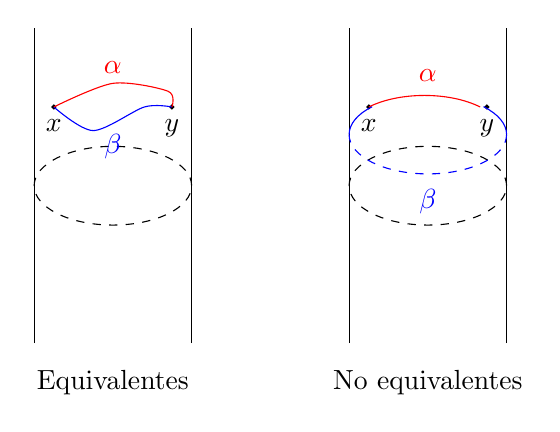
\begin{tikzpicture}
            \shorthandoff{>}

            % Cilindro 1
            \draw[dashed] (-3,0) ellipse (1 and 0.5);
            \draw (-4,-2) -- (-4,2);
            \draw (-2,-2) -- (-2,2);

            % Cilindro 2
            \draw[dashed] (1,0) ellipse (1 and 0.5);
            \draw (0,-2) -- (0,2);
            \draw (2,-2) -- (2,2);

            % Puntos x e y (1)
            \node[draw, circle, fill=black, inner sep=0.5pt, label=below:$x$] at (-3.75,1) {};
            \node[draw, circle, fill=black, inner sep=0.5pt, label=below:$y$] at (-2.25,1) {};

            % Arcos (1)
            \draw[blue] plot[smooth] coordinates {
                (-3.75,1) (-3.25,0.7) (-2.6,1)  (-2.25,1)
            };
            \draw[red] plot[smooth] coordinates {
                (-3.75,1) (-3,1.3) (-2.3,1.2)  (-2.25,1)
            };
            \node[red] at (-3,1.5) {$\alpha$};
            \node[blue] at (-3,0.5) {$\beta$};

            % Puntos x e y (2)
            \node[draw, circle, fill=black, inner sep=0.5pt, label=below:$y$] at (1.75,1) {};
            \node[draw, circle, fill=black, inner sep=0.5pt, label=below:$x$] at (0.25,1) {};

            % Arcos (2)
            \draw[blue, dashed] (2,0.65) arc (0:-180:1 and 0.5);
            \draw[blue] (2,0.65) arc (0:45:1 and 0.5);
            \draw[blue] (0,0.65) arc (180:135:1 and 0.5);
            \draw[red] (0.25,1) arc (135:45:1 and 0.5);
            \node[red] at (1,1.4) {$\alpha$};
            \node[blue] at (1,-0.2) {$\beta$};

            % Textos
            \node at (1,-2.5) {No equivalentes};
            \node at (-3,-2.5) {Equivalentes};

        \end{tikzpicture}
    \end{figure}

    \begin{proof}\
        \begin{enumerate}
            \item[(i)] Dado $\alpha \in \Omega(X;x,y)$ queremos ver que $\alpha$ es homotópica por arcos con $\alpha$. Para ello tenemos 
            \begin{align*}
                H(s,t) = \alpha(s) \hspace{1cm} & H(s,0) = \alpha(s)=H(s,1)\\
                H(0,t) = \alpha(0)=x \hspace{1cm} & H(1,t) = \alpha(1) = y
            \end{align*}

            \item[(ii)] Dados $\alpha, \beta\in \Omega(X;x,y)$ tales que existe $H:[0,1]\times [0,1]\to X$ continua tal que 
            \begin{align*}
                H(s,0) = \alpha(s) \hspace{0.5cm} &\text{ y } \hspace{0.5cm} H(s,1) = \beta(x) \ \ \ &\forall s\in [0,1]\\
                H(0,t) = x  \hspace{0.5cm} &\text{ y } \hspace{0.5cm} H(1,t) = y \ \ \ &\forall t \in [0,1]
            \end{align*}
            Queremos ver que existe un $\tilde{H}:[0,1]\times[0,1]\to X$ continua tal que 
            \begin{align*}
                \tilde{H}(s,0) = \beta(s) \hspace{0.5cm} &\text{ y } \hspace{0.5cm} \tilde{H}(s,1) = \alpha(x) \ \ \ &\forall s\in [0,1]\\
                \tilde{H}(0,t) = x  \hspace{0.5cm} &\text{ y } \hspace{0.5cm} \tilde{H}(1,t) = y \ \ \ &\forall t \in [0,1]
            \end{align*}
            Tomando $\tilde{H}(s,t):=H(s, 1-t)$ cumple claramente con lo que buscamos.

            \item[(iii)] Dado $\alpha, \beta, \gamma\in \Omega(X;x,y)$ y $H_1,H_2:[0,1]\times[0,1]\to X$ continuas tales que 
            \begin{gather*}
                \begin{array}{c c c c}
                    H_1(s,0) = \alpha(s) &&& H_2(s,0) = \beta(s)\\
                    H_1(s,1) = \beta(s) &&& H_2(s,1) = \gamma(s)\\
                    H_1(0,t) = x &&& H_2(0,t) = x\\
                    H_1(1, t) = x &&& H_2(1,t) = y
                \end{array}
            \end{gather*}
            Queremos ver que existe un $H:[0,1]\times [0,1]\to X$ tal que 
            \begin{align*}
                H(s,t) = \alpha(s) \hspace{1cm} & H(s,0) = \alpha(s)=H(s,1)\\
                H(0,t) = \alpha(0)=x \hspace{1cm} & H(1,t) = \alpha(1) = y
            \end{align*}
            Para ello consideramos 
            \begin{gather*}
                H(s,t) = \left\{
                    \begin{array}{l c c}
                        H_1(s,2t) & \text{ si } & 0 \leq t \leq \nicefrac{1}{2}\\
                        H_2(s, 2t-1) & \text{ si } & \nicefrac{1}{2} \leq t \leq 1
                    \end{array}
                \right.
            \end{gather*}
            Y con el lema de pegado es fácil ver que es continua y que satisface las condiciones que buscábamos.
        \end{enumerate}
    \end{proof}
\end{lema}

% TODO: Hacer lo mismo pero para homotopía

\begin{ejemplo}\
    \begin{enumerate}
        \item Sean $X$ un e.t. y $f,g:X \to \bb{R}^n$ aplicaciones continuas, entonces vamos a ver que $f$ y $g$ son homotópicas.
        \begin{proof}
            Vamos a definir la aplicación
            \begin{align*}
                H:X\times [0,1]&\to \bb{R}^n\\
                (x,t) & \mapsto (1-t)f(x) + tg(x)
            \end{align*} 
            que es continua y además verifica
            \begin{gather*}
                H(x,0) = f(x) \hspace{2cm} H(x,1) = g(x)
            \end{gather*}
            por lo que tenemos lo que buscábamos.
        \end{proof}
        En el caso particular de que $f=\alpha$ y $g=\beta$ fuesen arcos comenzando en un punto común y acabando en otro punto común, entonces la $H$ anterior sería una homotopía por arcos.

        \item Si $\alpha: [0,1]\to X$ es un arco y $h:[0,1] \to [0,1]$ es una aplicación continua con $h(0)=0$ y $h(1)=1$, entonces $\dot{\alpha}(s) = \alpha(h(s))$ es homotópica por arcos a $\alpha(s)$.
        
        \begin{proof}
            Es claro que $\dot{\alpha}$ es continua y existe una homotopía por arcos entre $\alpha$ y $\dot{\alpha}$ que es la siguiente
            \begin{gather*}
                H(s,t) = \alpha((1-t)s + th(s))
            \end{gather*}
            que es claramente continua y que verifica que 
            \begin{align*}
                H(s,0) = \alpha(s) \hspace{1cm} & H(s,1) = \alpha(h(s)) = \dot{\alpha}(s)\\
                H(0,t) = \alpha(0)=\dot{\alpha}(1) \hspace{1cm} & H(1,t) = \alpha(1) = \dot{\alpha}(1)
            \end{align*}
        \end{proof}
        Intuitivamente podemos entender esto como que no importa a qué velocidad se recorra una curva para ser homotópico por arcos.
    \end{enumerate} 
\end{ejemplo}

\begin{notacion}
    Como convenio a la clase de equivalencia de un arco $\alpha$ en $\Omega(X;x,y)$ lo denotaremos por $[\alpha]$.
\end{notacion}

\begin{lema}
    Dados dos arcos $\alpha_1, \alpha_2$ en $\Omega(X;x,y)$ y $\beta_1, \beta_2\in \Omega(X; y,z)$. Se verifica que si $[\alpha_1] = [\alpha_2]$, entonces $[\alpha_1\ast\beta_1] = [\alpha_2\ast\beta_2]$.

    \begin{proof}
        Tenemos que 
        \begin{gather*}
            (\alpha_1\ast\beta_1) = \left\{
                \begin{array}{l c c}
                    \alpha_1(2s) & \text{ si } & 0 \leq s \leq \nicefrac{1}{2}\\
                    \beta_1(2s-1) & \text{ si } & \nicefrac{1}{2} \leq s \leq 1
                \end{array}
            \right.\\\\
            (\alpha_2\ast\beta_2) = \left\{
                \begin{array}{l c c}
                    \alpha_2(2s) & \text{ si } & 0 \leq s \leq \nicefrac{1}{2}\\
                    \beta_2(2s-1) & \text{ si } & \nicefrac{1}{2} \leq s \leq 1
                \end{array}
            \right.
        \end{gather*}
        Además, sabemos que existen $H_1, H_2$ continuas tal que 
        \begin{gather*}
            \begin{array}{c c c c}
                H_1(s,0) = \alpha_1(s) &&& H_2(s,0) = \beta_1(s)\\
                H_1(s,1) = \beta_1(s) &&& H_2(s,1) = \beta_2(s)\\
                H_1(0,t) = x &&& H_2(0,t) = y\\
                H_1(1, t) = y &&& H_2(1,t) = z
            \end{array}
        \end{gather*}
        Tomamos entonces $H:[0,1]\times [0,1] \to X$ dada por 
        \begin{gather*}
            H(s,t) = \left\{
                \begin{array}{l c c}
                    H_1(2s, t) & \text{ si } & s \in [0,\nicefrac{1}{2}],\ t\in [0,1]\\
                    H_2(2s-1, t) & \text{ si } & s \in [\nicefrac{1}{2},1],\ t\in [0,1]\\
                \end{array}
            \right.
        \end{gather*}
        es continua y tenemos que 
        \begin{gather*}
            H(s,0) = \left\{
                \begin{array}{l c c}
                    H_1(2s, 0) & \text{ si } & s \in [0,\nicefrac{1}{2}]\\
                    H_2(2s-1, 0) & \text{ si } & s \in [\nicefrac{1}{2},1]\\
                \end{array}
            \right. = 
            \left\{
                \begin{array}{l c c}
                    \alpha_1(2s) & \text{ si } & s \in [0,\nicefrac{1}{2}]\\
                    \beta_1(2s-1) & \text{ si } & s \in [\nicefrac{1}{2},1]\\
                \end{array}
            \right. = (\alpha_1 \ast \beta_1)(s)
        \end{gather*}
        Análogamente se tiene que $H(s,1)=(\alpha_2\ast\beta_2)(s)$ con $H(0,t) = x$ y $H(1,t) = z$.

    \end{proof}
    A partir del lema anterior podemos definir
    \begin{gather*}
        [\alpha] \ast [\beta] := [\alpha \ast \beta]
    \end{gather*}
    con $\alpha\in \Omega(X;x,y)$, $\beta \in \Omega(X;y,z)$
\end{lema}

\begin{teo}
    Dado $X$ e.t., $\alpha\in \Omega(X;x,y)$, $\beta\in \Omega(X;y,z)$ y $\gamma\in \Omega(X;z,w)$ se tiene que 
    \begin{enumerate}
        \item[(i)] $[\alpha] \ast ([\beta] \ast [\gamma]) = ([\alpha] \ast [\beta]) \ast [\gamma]$
        \item[(ii)] $[\alpha]\ast [\veps_y] = [\alpha]$ y $[\veps_x]\ast [\alpha] = [\alpha]$
        \item[(iii)]  $[\alpha]\ast [\tilde{\alpha}] = [\veps_x]$ y $[\tilde{\alpha}]\ast [\alpha] = [\veps_y]$
    \end{enumerate}
    \begin{proof}\
        \begin{enumerate}
            \item[(i)] Desarrollemos cada expresión
            \begin{figure}[H]
                \centering
                \begin{tikzpicture}
                    \shorthandoff{>}

                    % Líneas discontinuas
                    \draw[gray!50, dashed] (0,-1) -- (0,2);
                    \draw[gray!50, dashed] (4,-1) -- (4,2);
                    \draw[gray!50, dashed] (8,-1) -- (8,2);
                    \draw[gray!50, dashed] (12,-1) -- (12,2);
                    
                    % Puntos
                    \node[draw, circle, fill=black, inner sep=0.5pt, label=below:$x$] at (0,0) {};
                    \node[draw, circle, fill=black, inner sep=0.5pt, label=below:$y$] at (4,1) {};
                    \node[draw, circle, fill=black, inner sep=0.5pt, label=below:$z$] at (8,0.8) {};
                    \node[draw, circle, fill=black, inner sep=0.5pt, label=below:$w$] at (12,1) {};

                    % Arcos
                    \draw[blue] plot[smooth, tension=1] coordinates {
                        (0,0) (2,1) (4,1)
                    };
                    \draw[red] plot[smooth, tension=1] coordinates {
                        (4,1) (6,0.6) (8,0.8)
                    };
                    \draw[green!60!black] plot[smooth, tension=1] coordinates {
                        (8,0.8) (9,1) (10.6,0.6) (12,1)
                    };

                    % Nombre arcos
                    \node[blue] at (2,1.3) {$\alpha$};
                    \node[red] at (6,0.9) {$\beta$};
                    \node[green!60!black] at (10,1) {$\gamma$};

                    % Leyenda tiempos
                    \node at (0,-1.2) {$s=0$};
                    \node[violet] at (4,-1.2) {$s=\nicefrac{1}{4}$};
                    \node[violet] at (8,-1.2) {$s=\nicefrac{1}{2}$};
                    \node[orange!90!black] at (4,-1.7) {$s=\nicefrac{1}{2}$};
                    \node[orange!90!black] at (8,-1.7) {$s=\nicefrac{3}{4}$};
                    \node at (12,-1.2) {$s=1$};

                    % Leyenda colores
                    \draw[violet] (13,2)--(13.5,2);
                    \draw[orange!90!black] (13,0)--(13.5,0);
                    \node[anchor=west, text width=2.2cm, align=center] at (13.7,2) {Tiempos de \\$(\alpha\ast\beta)\ast\gamma$};
                    \node[anchor=west, text width=2.2cm, align=center] at (13.7,0) {Tiempos de \\$\alpha\ast(\beta\ast\gamma)$};

                \end{tikzpicture}
            \end{figure}
            \begin{align*}
                (\beta\ast\gamma)(s) &= \left\{
                    \begin{array}{l c c}
                        \beta(2s) & \text{ si } & s \in [0,\nicefrac{1}{2}]\\
                        \gamma(2s-1) & \text{ si } & s \in [\nicefrac{1}{2},1]\\
                    \end{array}
                \right.\\\\
                \alpha \ast(\beta\ast\gamma)(s) &= \left\{
                    \begin{array}{l c c}
                        \alpha(2s) & \text{ si } & s \in [0,\nicefrac{1}{2}]\\
                        (\beta\ast\gamma)(2s-1) & \text{ si } & s \in [\nicefrac{1}{2},1]\\
                    \end{array}
                \right. =\\
                &= \left\{
                    \begin{array}{l c c}
                        \alpha(2s) & \text{ si } & s \in [0,\nicefrac{1}{2}]\\
                        \beta(2(2s-1)) & \text{ si } & s \in [\nicefrac{1}{2},\nicefrac{3}{4}]\\
                        \gamma(2(2s-1)-1) & \text{ si } & s \in [\nicefrac{3}{4},1]\\
                    \end{array}
                \right. = \left\{
                    \begin{array}{l c c}
                        \alpha(2s) & \text{ si } & s \in [0,\nicefrac{1}{2}]\\
                        \beta(4s-2) & \text{ si } & s \in [\nicefrac{1}{2},\nicefrac{3}{4}]\\
                        \gamma(4s-3) & \text{ si } & s \in [\nicefrac{3}{4},1]\\
                    \end{array}
                \right.\\\\\\
                %
                %
                %
                (\alpha\ast\beta)(s) &= \left\{
                    \begin{array}{l c c}
                        \alpha(2s) & \text{ si } & s \in [0,\nicefrac{1}{2}]\\
                        \beta(2s-1) & \text{ si } & s \in [\nicefrac{1}{2},1]\\
                    \end{array}
                \right.\\\\
                (\alpha \ast\beta)\ast\gamma(s) &= \left\{
                    \begin{array}{l c c}
                        (\alpha\ast\beta)(2s) & \text{ si } & s \in [0,\nicefrac{1}{2}]\\
                        \gamma(2s-1) & \text{ si } & s \in [\nicefrac{1}{2},1]\\
                    \end{array}
                \right. =\\
                &= \left\{
                    \begin{array}{l c c}
                        \alpha(2(2s)) & \text{ si } & s \in [0,\nicefrac{1}{4}]\\
                        \beta(2(2s)-1) & \text{ si } & s \in [\nicefrac{1}{4},\nicefrac{1}{2}]\\
                        \gamma(2s-1) & \text{ si } & s \in [\nicefrac{3}{4},1]\\
                    \end{array}
                \right. = \left\{
                    \begin{array}{l c c}
                        \alpha(4s) & \text{ si } & s \in [0,\nicefrac{1}{4}]\\
                        \beta(4s-1) & \text{ si } & s \in [\nicefrac{1}{4},\nicefrac{1}{2}]\\
                        \gamma(2s-1) & \text{ si } & s \in [\nicefrac{1}{2},1]\\
                    \end{array}
                \right.
            \end{align*}

            Usando el ejemplo 2 anterior se tiene que $[\alpha] \ast ([\beta] \ast [\gamma]) = ([\alpha] \ast [\beta]) \ast [\gamma]$ (realmente se están recorriendo las mismas curvas pero a distinta velocidad).


            \item[(ii)] Tendremos que ver que $\alpha \ast \veps_y$ se relaciona por una homotopía con arcos con $\alpha$. Recordemos que
            \begin{gather*}
                (\alpha \ast \veps_y) = \left\{
                    \begin{array}{l c c}
                        \alpha(2s) & \text{ si } & 0\leq s \leq \nicefrac{1}{2} \\
                        \veps_y(2s-1) & \text{ si } & \nicefrac{1}{2} \leq s \leq 1
                    \end{array}
                \right. = 
                \left\{
                    \begin{array}{l c c}
                        \alpha(2s) & \text{ si } & 0\leq s \leq \nicefrac{1}{2} \\
                        y & \text{ si } & \nicefrac{1}{2} \leq s \leq 1
                    \end{array}
                \right.
            \end{gather*}
            De nuevo del ejemplo 2 se tiene que son homotópicas

            \item[(iii)] Tendremos que ver en este caso que $\alpha\ast\tilde{\alpha}$ es homotópico por arcos a $\veps_x$. Describamos ambas curvas.
            \begin{gather*}
                (\alpha \ast \tilde{\alpha}) = \left\{
                    \begin{array}{l c c}
                        \alpha(2s) & \text{ si } & 0\leq s \leq \nicefrac{1}{2} \\
                        \tilde{\alpha}(2s-1) & \text{ si } & \nicefrac{1}{2} \leq s \leq 1
                    \end{array}
                \right. = \left\{
                    \begin{array}{l c c}
                        \alpha(2s) & \text{ si } & 0\leq s \leq \nicefrac{1}{2} \\
                        \tilde{\alpha}(2-2s) & \text{ si } & \nicefrac{1}{2} \leq s \leq 1
                    \end{array}
                \right.\\\\
                \veps_x(s) = x \ \ \ \forall s \in [0,1]
            \end{gather*}
            Pensamos ahora una transformación $H$ que haga que cada vez la curva se vaya quedando más cerca de $x$ (cada vez vuelve antes de llegar a $y$). Intuitivamente podríamos pensar en la siguiente gráfica, en la que vamos reduciendo la distancia desde la función roja hasta la verde
            \begin{figure}[H]
                \centering
                \begin{tikzpicture}[scale=0.75]
                    \begin{axis}[
                        axis lines=left,
                        height=8cm, width=10cm,
                        xmin=-0.2, xmax=1.2,
                        ymin=-0.2, ymax=1.2,
                        xtick={0,0.5,1},
                        ytick={0,1},
                        xticklabels={$0$, $\tfrac{1}{2}$, $1$},
                        yticklabels={$0$,$1$},
                        grid=major,
                        axis x line=middle, % eje X en y=0
                        axis y line=middle, % eje Y en x=0
                        xlabel={$s$},       % nombre eje X
                        ylabel={$t$},       % nombre eje Y
                        xlabel style={below},  % opcional: ajustar posición
                        ylabel style={left},  % opcional: ajustar posición
                    ]
                        % Líneas
                        \addplot[very thick,red!60!black] coordinates {(0,0) (0.5,1) (1,0)};
                        \addplot[very thick,blue!60!black] coordinates {(0,0) (0.5,0.8) (1,0)};
                        \addplot[very thick,yellow] coordinates {(0,0) (0.5,0.3) (1,0)};
                        \addplot[very thick,green!60!black] coordinates {(0,0.01) (0.5,0.01) (1,0.01)};
                    \end{axis}
                \end{tikzpicture}%
            \end{figure}%
            \begin{gather*}
                h(s) = \left\{
                    \begin{array}{l c c}
                        2s & \text{ si } & s\in [0,\nicefrac{1}{2}]\\
                        2-2s & \text{ si } & s\in [\nicefrac{1}{2}, 1]
                    \end{array}
                \right. 
            \end{gather*}
            Y podemos construir $H(s,t) = \alpha((1-t)h(s))$ que claramente es continua y verifica
            \begin{align*}
                H(s,0) = \alpha(h(s)) = (\alpha\ast\tilde{\alpha}(s)) \hspace{0.5cm} &\text{ y } \hspace{0.5cm} H(s,1) = \alpha(0) = x = \veps_x(s) \ \ \ &\forall s\in [0,1]\\
                H(0,t) = \alpha(0) = x  \hspace{0.5cm} &\text{ y } \hspace{0.5cm} H(1,t) = \alpha(0) = x \ \ \ &\forall t \in [0,1]
            \end{align*}
        \end{enumerate}
    \end{proof}

    \section{El grupo fundamental}
    \begin{coro}
        Dados un e.t. $X$ y un punto $x_0\in X$ se tiene que el conjunto de lazos en $X$ basados en $x_0$ bajo la relación de equivalencia de ser homotópicos por arcos y con operación $\ast$ forman un grupo algebraico.

        \begin{proof}
            Definimos el siguiente conjunto
            \begin{gather*}
                G = \frac{\Omega(X;x_0)}{R}
            \end{gather*}
            donde $R$ es la relación de equivalencia ``ser homotópico por arcos''. Veamos ahora que $G$ tiene estructura de grupo:
            \begin{enumerate}
                \item \textbf{Propiedad asociativa.} Tendremos que ver que se verifica para cualesquiera $[\alpha],[\beta], [\gamma]\in G$.
                \begin{gather*}
                    [\alpha] \ast ([\beta] \ast [\gamma]) = ([\alpha] \ast [\beta]) \ast [\gamma]
                \end{gather*}
                pero esto lo tenemos claramente del teorema anterior

                \item \textbf{Existencia del elemento neutro.} Por el teorema anterior tenemos que para $x=y=x_0$ se tiene que $[\alpha] \ast [\veps_{x_0}] = [\alpha] = [\veps_{x_0}] \ast [\alpha]$ para cualquier $[\alpha]\in G$ luego tenemos la existencia probada.
                \item \textbf{Existencia del elemento opuesto.} De nuevo usamos el teorema anterior y nos dice que para cualquier $[\alpha]\in G$ se tiene que 
                \begin{gather*}
                    [\alpha] \ast [\tilde{\alpha}] = [\veps_{x_0}] =  [\tilde{\alpha}] \ast [\alpha] 
                \end{gather*}
                y se tiene directamente.
            \end{enumerate}
            Con esto hemos probado finalmente que $G$ es un grupo.
        \end{proof}
    \end{coro}
\end{teo}

\begin{definicion}
    Al grupo algebraico dado por el corolario anterior lo llamaremos el \textbf{grupo fundamental} de $X$ en $x_0$ y lo denotaremos por $\pi_1(X,x_0)$.
\end{definicion}

\begin{ejemplo} Consideramos $\bb{R}^2\setminus \{0,0\}$ y un punto cualquiera $x_0$.

    \begin{figure}[H]
        \centering
        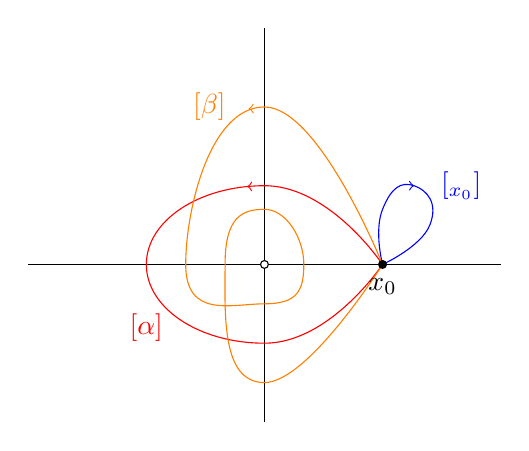
\begin{tikzpicture}
            \shorthandoff{>}

            % Ejes
            \draw (-3,0) -- (3,0);
            \draw (0,-2) -- (0,3);

            % Arcos
            \draw[blue] plot[smooth, tension=1] coordinates {
                (1.5,0) (1.5,0.7) (1.9,1) (2.1,0.5) (1.5,0)
            };
            \draw[->, blue] (1.9,1) ++(-0.01, 0) -- ++(0.01,0);


            \draw[red] plot[smooth, tension=1] coordinates {
                (1.5,0) (0,1) (-1.5,0) (0,-1) (1.5,0)
            };
            \draw[->, red] (-0.22,0.99) ++(+0.01, 0) -- ++(-0.01,0);

            \draw[orange] plot[smooth, tension=1] coordinates {
                (1.5,0) (0,2) (-1,0) (0,-0.5) (0.5,0) (0,0.7) (-0.5, 0) (0,-1.5) (1.5,0)
            };
            \draw[->, orange] (-0.2,1.98) ++(+0.01, 0) -- ++(-0.01,0);

            % Leyendas
            \node[blue] at (2.5,1) {$[\veps_{x_0}]$};
            \node[red] at (-1.5, -0.8) {$[\alpha]$};
            \node[orange] at (-0.7, 2) {$[\beta]$};

            % Puntos
            \node[draw, circle, fill=white, inner sep=1pt] at (0,0) {};
            \node[draw, circle, fill=black, inner sep=1pt, label=below:$x_0$] at (1.5,0) {};

        \end{tikzpicture}%
    \end{figure}%

    En este espacio tenemos que $[\veps_{x_0}] \neq [\alpha] \neq [\tilde{\alpha}] \neq [\beta]$. Intuitivamente podríamos intentar identificar este espacio con $\bb{Z}$ de la siguiente forma:
    
    \begin{itemize}
        \item La clase $[\veps_{x_0}]$ la podemos interpretar como el $0$ de $\bb{Z}$.
        \item Identificaremos los números positivos como el número de vueltas que da cada curva al punto $(0,0)$ en sentido positivo (el que elijamos como positivo). Por ejemplo $[\alpha]$ sería $1\in \bb{Z}$, $[\beta]$ sería $2\in \bb{Z}$ y podríamos seguir así con todos los números enteros.
        \item Para los números negativos tomaremos los opuestos de los anteriores, es decir, las curvas recorridas en sentido contrario. Por ejemplo $[\tilde{\alpha}]$ será el $-1\in \bb{Z}$, $[\tilde{\beta}]$ será el $-2$ y así sucesivamente. 
    \end{itemize}

    Más adelante probaremos que $\pi_1(X,x_0)$ es isomorfo a $\bb{Z}$ de una forma más rigurosa.
\end{ejemplo}

\begin{ejemplo}
    Sea $X\subseteq \bb{R}^n$ un subconjunto estrellado desde un punto $x_0$. Entonces $\pi_1(X;x_0) = \{[\veps_{x_0}]\}$, es decir, es trivial.

    \begin{proof}
        Dado $\alpha(s)$ un lazo basado en $x_0$ dentro de $X$, entonces 
        \begin{gather*}
            H(s,t) = (1-t)\alpha(s)+tx_0
        \end{gather*}
        es una aplicación continua dentro\footnote{aquí es donde usamos que es estrellado} de $X$ tal que 
        \begin{align*}
            H(s,0) = \alpha(s) = \hspace{0.5cm} &\text{ y } \hspace{0.5cm} H(s,1) = x_0 = \veps_{x_0}(s) \ \ \ &\forall s\in [0,1]\\
            H(0,t) = x_0  \hspace{0.5cm} &\text{ y } \hspace{0.5cm} H(1,t) = x_0\ \ \ &\forall t \in [0,1]
        \end{align*}
    \end{proof}
    En particular, las bolas abiertas, las bolas cerradas, los convexos en general como $\bb{R}^n$ tienen grupo fundamental trivial.
\end{ejemplo}

\begin{teo}
    Sean $x,y$ dos puntos de un e.t. $X$. Si $X$ es arcoconexo, entonces $\pi_1(X,x)$ y $\pi_1(X,y)$ son iguales salvo isomorfismo.
    \begin{proof}
        Como $X$ es arcoconexo podemos considerar $\alpha$ un arco uniendo $x$ con $y$ y la aplicación
        \begin{align*}
            F_\alpha : \pi_1(X,y) &\to \pi_1(X,x)\\
            [\gamma] & \mapsto [\alpha]\ast[\gamma]\ast[\tilde{\alpha}]
        \end{align*}
        que está bien definida por lo visto anteriormente sobre el operador $\ast$. Queremos ver ahora que $F_\alpha$ es un isomorfismo de grupos. Para ello comencemos por ver que $F_\alpha$ es un homomorfismo, es decir, que se verifica
        \begin{gather*}
            F_\alpha([\gamma_1] \ast [\gamma_2]) = F_\alpha[\gamma_1]\ast F_\alpha([\gamma_2])
        \end{gather*}
        Desarrollamos el segundo término de la expresión:
        \begin{align*}
            F_\alpha[\gamma_1]\ast F_\alpha([\gamma_2]) &= ([\alpha] \ast [\gamma_1] \ast [\tilde{\alpha}]) \ast ([\alpha] \ast [\gamma_2] \ast [\tilde{\alpha}]) = [\alpha] \ast [\gamma_1] \ast [\gamma_2] \ast [\tilde{\alpha}] =\\
            &= F_\alpha([\gamma_1] \ast [\gamma_2])
        \end{align*}
        y tenemos la igualdad buscada. Veamos ahora que tiene inversa considerando $F_{\tilde{\alpha}}$ que por definición es $F_{\tilde{\alpha}}([\beta]) = [\tilde{\alpha}] \ast [\beta] \ast [\alpha]$ y que además verifica
        \begin{gather*}
            (F_{\tilde{\alpha}} \circ F_{\tilde{\alpha}})([\gamma]) = F_{\tilde{\alpha}}([\alpha]\ast [\gamma]\ast [\tilde{\alpha}]) = [\tilde{\alpha}] \ast ([\alpha]\ast [\gamma]\ast [\tilde{\alpha}]) \ast [\alpha] = [\gamma] = Id_{\pi_1(X,y)}([\gamma])\\
            %
            (F_\alpha \circ F_{\tilde{\alpha}})([\gamma]) = F_\alpha([\tilde{\alpha}] \ast [\gamma] \ast [\alpha]) = [\alpha] \ast ([\tilde{\alpha}] \ast [\gamma] \ast [\alpha]) \ast [\tilde{\alpha}] = [\gamma] = Id_{\pi_1(X,x)}([\gamma])
        \end{gather*}
        por lo que es su inversa. Hemos encontrado por tanto un homomorfismo biyectivo, luego $\pi_1(X,x) \cong \pi_1(X,y)$
    \end{proof}
\end{teo}

\begin{definicion}
    Decimos que un e.t. es \textbf{simplemente conexo} si es arcoconexo y su grupo fundamental es el trivial en un punto (y, por tanto, en cualquier punto).
\end{definicion}

\begin{ejemplo}
    Si $A\subset \bb{R}^n$ es estrellado desde un punto $x_0$, entonces $A$ es simplemente conexo.
\end{ejemplo}

\begin{lema}
    Sea $f:X\to Y$ una aplicación continua entre espacios topológicos y $x\in X$. Entonces la aplicación
    \begin{align*}
        (f_x)_* : \pi_1(X,x) &\to \pi_1(Y,f(x))\\
        [\alpha] &\mapsto [f\circ \alpha]
    \end{align*}
    está bien definida y es un homomorfismo de grupos\footnote{Cuando no haya confusión posible escribiremos solamente $f_*$ en lugar de $(f_x)_*$}.

    \begin{proof}
        Para ver que $(f_x)_*$ está bien definida tomamos $\alpha_1,\ \alpha_2$ lazos basados en $x$ tales que $[\alpha_1] = [\alpha_2]$. Queremos comprobar que $[f\circ \alpha_1] = [f\circ \alpha_2]$. Para ello , sabemos que si $[\alpha_1] = [\alpha_2]$, entonces existe $H:[0,1]\to X$ continua y tal que
        \begin{gather*}
            H(s,0) =\alpha_1(s)\ \ \  ,\ \ \ H(s,1) = \alpha_2(s)\ \ \ , \ \ \ H(0,t)=x=H(1,t)
        \end{gather*}
        Entonces podemos considerar la aplicación 
        \begin{align*}
            f\circ H : [0,1]\times [0,1] \to Y
        \end{align*}
        que es continua y verifica 
        \begin{gather*}
            (f\circ H) (s,0) = (f \circ \alpha_1)(s)\\
            (f\circ H) (s,1) = (f\circ \alpha_2)(s)\\
            (f\circ H) (0,t) = f(x) = (f\circ H) (1,t)
        \end{gather*}
        por lo que $[f\circ \alpha_1] = [f\circ \alpha_2]$. Veamos ahora que $(f_x)_*$ es un homomorfismo de grupos, es decir que se verifica
        \begin{gather*}
            (f_x)_* ([\alpha] \ast [\beta] ) = (f_x)_* ([\alpha]) \ast (f_x)_* ([\beta])
        \end{gather*}
        Por definición sabemos que 
        \begin{gather*}
            (f_x)_* ([\alpha] \ast [\beta] ) = (f_x)_*([\alpha \ast \beta]) = [f\circ(\alpha \ast \beta)] = \left[\left\{
                \begin{array}{l c c}
                    f(\alpha(2s)) & \text{ si } & 0\leq s \leq \nicefrac{1}{2}\\
                    f(\beta(2s-1)) & \text{ si } & \nicefrac{1}{2} \leq s \leq 1\\
                \end{array}
            \right.\right]=\\
            =[(f\ast \alpha) \ast (f\circ \beta)] = (f_x)_* ([\alpha]) \ast (f_x)_* ([\beta])
        \end{gather*}
    \end{proof}
\end{lema}

\begin{definicion}
    A la aplicación $f_x$ dada por el lema la llamaremos \textbf{homomorfismo inducido} por $f$.
\end{definicion}

\begin{propiedades}
    Algunas propiedades básicas de $f_x$ son
    \begin{enumerate}
        \item Si tenemos dos aplicaciones continuas $f:X\to Y$ y $g:Y \to Z$, entonces se tiene que 
        \begin{gather*}
            (g\circ f)_* = g_x \circ f_x
        \end{gather*}

        \item  Se verifica que la aplicación dada por
        \begin{align*}
            Id_x: \pi_1(X,x_0) &\to \pi(X,x_0)\\
            [\alpha] & \mapsto [\alpha]
        \end{align*}
        es la identidad en grupos fundamentales.
    \end{enumerate}
\end{propiedades}

\begin{coro}
    Si $h:X\to Y$ es un homeomorfismo, entonces la aplicación dada por
    \begin{gather*}
        (h_x)_*:\pi_1(X,x) \to \pi_1(Y,h(x))
    \end{gather*}
    es un isomorfismo de grupos, es decir, el grupo fundamental se conserva\footnote{salvo isomorfismo} por homeomorfismos.
\end{coro}

\begin{definicion}
    Si $(G_1,\ast_1)$ y $(G_2, \ast_2)$ son dos grupos algebraicos, consideramos sobre $G_1\times G_2$ el producto $\ast$ dado por 
    \begin{gather*}
        (a_1,b_1)\ast(a_2,b_2) := (a_1\ast_1 a_2, b_1 \ast_2 b_2)
    \end{gather*}
    para $a_1,a_2\in G_1$, $b_1,b_2\in G_2$
\end{definicion}

\begin{teo}
    Sean $X,Y$ dos e.t., $x\in X$, $y\in Y$. Entonces, con la topología producto en $X\times Y$ se tiene que 
    \begin{gather*}
        \pi_1(X\times Y, (x,y)) \cong \pi_1(X,x) \times \pi_1(Y,y)
    \end{gather*}
    \begin{proof}
        Veasmos que 
        \begin{align*}
            \phi: \pi_1(X\times Y,(x,y)) &\longrightarrow \pi_1(X,x) \times \pi_1(Y,y) \\
            [\alpha] & \longmapsto ([p_1 \circ \alpha], [p_2\circ \alpha])
        \end{align*}
        donde $p_1$ y $p_2$ son las proyecciones a $X$ y a $Y$ respectivamente está bien definida. Esto es fácil de ver ya que 
        \begin{gather*}
            ([p_1 \circ \alpha], [p_2\circ \alpha]) = ((p_1)_*([\alpha]), (p_2)_*([\alpha]))
        \end{gather*}
        y además es un homomorfismo. Consideramos además la siguiente aplicación
        \begin{align*}
            \psi: \pi_1(X,x)\times \pi_1(Y,y) \longrightarrow \pi_1(X\times Y, (x,y))\\
            ([\beta], [\gamma]) & \longmapsto [(\beta, \gamma)]
        \end{align*}
        y es fácil ver que está bien definida y es un homomorfismo tal que
        \begin{gather*}
            \psi \circ \phi = Id_{\pi_1(X\times Y,(x,y))}\\
            \phi \circ \psi = Id_{\pi_1(X,x) \times \pi_1(Y,y)}
        \end{gather*}
    \end{proof}
\end{teo}

\section{Espacios recubridores}

\begin{definicion}
    Sea $p:R\to B$ una aplicación continua y sobreyectiva entre dos espacios topológicos. Dado un punto $b\in B$ decimos que un abierto $O$ que contiene a $b$ está \textbf{regularmente recubierto} si se verifican las siguientes propiedades
    \begin{enumerate}
        \item $p^{-1}(O)$ es una unión disjunta de abiertos $A_i\subseteq R$, $i\in I$.
        \item Para cada $i\in I$, $p_{|A_i}:A_i \to O$ es un homeomorfismo.
    \end{enumerate}
\end{definicion}

\begin{ejemplo} 
    En este caso, si consideramos la aplicación $p:\bb{R} \to \bb{S}^1$ descrita en la gráfica, que es claramente continua y sobreyectiva\footnote{de hecho es un homeomorfismo que estudiamos en Topología I} podemos ver que $O$, que contiene al $(1,0)$ está regularmente recubierto

    \begin{figure}[H]
        \centering
        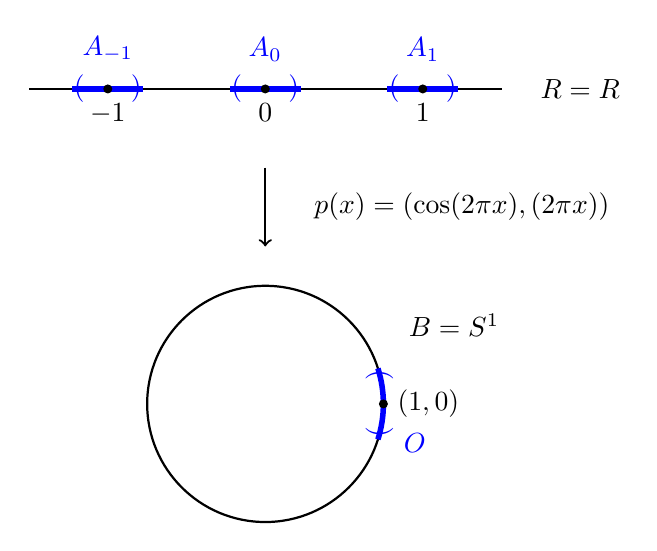
\begin{tikzpicture}
            \shorthandoff{>}

            % Recta
            \draw[line width=1pt] (-3,3) -- (3,3);
            \node at (4,3) {$R = \bb{R}$};

            % Abiertos en preimagen
            \node[blue] at (-2,3) {$(\ \ \ \ \ )$};
            \node[blue] at (0,3) {$(\ \ \ \ \ )$};
            \node[blue] at (2,3) {$(\ \ \ \ \ )$};

            \draw[line width=2pt, blue] (-2.45, 3) -- (-1.55, 3);
            \draw[line width=2pt, blue] (-0.45, 3) -- (0.45, 3);
            \draw[line width=2pt, blue] (2.45, 3) -- (1.55, 3);

            \node[blue] at (-2,3.5) {$A_{-1}$};
            \node[blue] at (0,3.5) {$A_{0}$};
            \node[blue] at (2,3.5) {$A_{1}$};

            % Puntos
            \node[draw, circle, fill=black, inner sep=1pt, label=below:$-1$] at (-2,3) {};
            \node[draw, circle, fill=black, inner sep=1pt, label=below:$0$] at (0,3) {};
            \node[draw, circle, fill=black, inner sep=1pt, label=below:$1$] at (2,3) {};

            % Flecha función
            \draw[line width=0.8pt,->] (0,2) -- (0,1);
            \node[anchor=west] at (0.5,1.5) {$p(x) = (\cos(2\pi x), \sen(2\pi x))$};

            % Circunferencia
            \draw[thick] (0,-1) circle [radius=1.5];
            \node[anchor=west] at (1.7,0) {$B=\bb{S}^1$};
            \node[rotate=90, blue] at (1.45,-1) {$(\ \ \ \ \ )$};
            \draw[blue, line width=2pt] (1.5,-1) arc (0:17.5:1.5);
            \draw[blue, line width=2pt] (1.5,-1) arc (0:-17.5:1.5);
            \node[draw, circle, fill=black, inner sep=1pt, label=right:{$(1,0)$}] at (1.5,-1) {};
            \node[blue] at (1.9,-1.5) {$O$};

        \end{tikzpicture}%
    \end{figure}%
\end{ejemplo}

\begin{definicion}
    Decimos que una aplicación $p:R \to B$ entre dos espacios topológicos es una \textbf{aplicación recubridora} si $p$ es continua, sobreyectiva y todo punto $b \in B$ está contenido en un abierto $O_b$ regularmente recubierto.
\end{definicion}

\begin{observacion}
    Todo homeomorfismo es una aplicación recubridora\footnote{Podemos verlo fácilmente tomando $O_b = X$ el total.}. 
\end{observacion}

\begin{teo}
    La aplicación
    \begin{align*}
        p:\bb{R} & \to \bb{S}^1\\
        x & \mapsto (\cos(2\pi x), \sen (2\pi x))
    \end{align*}
    es una aplicación recubridora
    \begin{proof}
        Es claro que es sobreyectiva y continua por las propiedades del seno y el coseno en $\bb{R}$. Tendremos que ver que 
        \begin{gather*}
            O=\bb{S}^1\cap ((0,\infty)\times \bb{R}) = \bb{S}^1 \cap \{(x_1,x_2)\in \bb{R}^2 : x_1>0\}
        \end{gather*}
        está regularmente recubierto. Para ello consideramos
        \begin{align*}
            p^{-1}(O) &= \{x\in \bb{R}: \cos(2\pi x) > 0\} = \{x\in \bb{R} : 2\pi x \in \left(-\frac{\pi}{2} + 2k\pi, \frac{\pi}{2} +2k\pi\right),\ k\in \bb{Z}\} =\\
            &=\{x\in \bb{R} : x \in \left(k-\frac{1}{4}, k+\frac{1}{4}\right),\ k\in \bb{Z}\} = \bigcup\limits_{k\in \bb{Z}}\left(k-\frac{1}{4}, k+\frac{1}{4}\right)
        \end{align*}
        Tomando $A_k = \left(k-\frac{1}{4}, k+\frac{1}{4}\right)$ falta ver que cada abierto $A_{k_0}$ cumple que $p:A_{k_0} \to O$ es un homeomorfismo.\\

        Por las propiedades de $(\cos(2\pi x), \sen(2\pi x))$ es claro que $p$ es inyectiva y sobreyectiva en $A_{k_0}$. Para ello podemos considerar 
        \begin{align*}
            p':\left[k-\frac{1}{4}, k+\frac{1}{4}\right] \to \overline{O}
        \end{align*}
        que es continua y va desde un compacto en un conjunto T2, lo que nos dice que $p_{|_{\left[k-\frac{1}{4}, k+\frac{1}{4}\right]}}$ es cerrada por lo que
        \begin{gather*}
            p':\left[k-\frac{1}{4}, k+\frac{1}{4}\right] \to \overline{O}
        \end{gather*}
        es un homeomorfismo y por tanto
        \begin{gather*}
            p':\left(k-\frac{1}{4}, k+\frac{1}{4}\right) \to \overline{O}
        \end{gather*}
        también lo es y como por la definición de $A_k$ tenemos lo que buscábamos. \\

        Si repetimos este razonamiento de forma análoga para los siguientes conjuntos:
        \begin{gather*}
            \bb{S}^1\cap \{(x_1,x_2)\in \bb{R}^2 : x_1<0\}\\
            \bb{S}^1\cap \{(x_1,x_2)\in \bb{R}^2 : x_2>0\}\\
            \bb{S}^1\cap \{(x_1,x_2)\in \bb{R}^2 : x_2<0\}
        \end{gather*}
        tendremos la demostración completa.
    \end{proof}
\end{teo}

\begin{ejemplo}
    La aplicación
    \begin{align*}
        p:\bb{S}^1 & \to \bb{S}^1\\
        (x,y) & \mapsto (x^2-y^2, 2xy)
    \end{align*}
    que podemos entender como la aplicación que lleva
    \begin{align*}
        (x+iy) &\mapsto (x+iy)^2\\
        (\cos \theta, \sen \theta) &\mapsto (\cos 2\theta, \sen 2\theta)
    \end{align*}
    es recubridora. Intuitivamente la podemos ver como\\

    \begin{figure}[H]
        \centering
        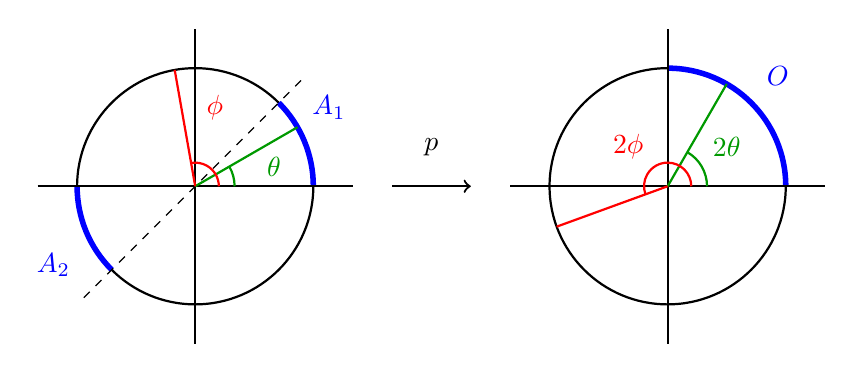
\begin{tikzpicture}
            \shorthandoff{>}

            % Aplicación p
            \node at (0,0.5) {$p$};
            \draw[thick,->] (-0.5,0) -- (0.5,0);

            % Circunferencia 1
            \draw[thick] (-3,0) circle [radius=1.5];
            \draw[blue, line width=2pt] (-1.5,0) arc (0:45:1.5);
            \draw[blue, line width=2pt] (-4.5,0) arc (180:225:1.5);
            
            \node[blue] at (-1.3,1) {$A_1$};
            \node[blue] at (-4.8,-1) {$A_2$};

            % Ejes 1
            \draw[thick] (-3,-2) -- (-3,2);
            \draw[thick] (-5,-0) -- (-1,0);
            \draw[rotate around={45:(-3,0)}, dashed] (-5,-0) -- (-1,0);

            \draw[thick, green!60!black, rotate around={30:(-3,0)}] (-3,0) -- (-1.5,0);
            \draw[thick, red, rotate around={100:(-3,0)}] (-3,0) -- (-1.5,0);

            \draw[green!60!black, thick] (-2.5,0) arc (0:30:0.5);
            \draw[red, thick] (-2.7,0) arc (0:100:0.3);

            \node[green!60!black] at (-2,0.25) {$\theta$};
            \node[red] at (-2.75,1) {$\phi$};

            % Circunferencia 2
            \draw[thick] (3,0) circle [radius=1.5];
            \draw[blue, line width=2pt] (4.5,0) arc (0:90:1.5);

            \node[blue] at (4.4,1.4) {$O$};

            % Ejes 2
            \draw[thick] (3,-2) -- (3,2);
            \draw[thick] (1,-0) -- (5,0);

            \draw[thick, green!60!black, rotate around={60:(3,0)}] (3,0) -- (4.5,0);
            \draw[thick, red, rotate around={200:(3,0)}] (3,0) -- (4.5,0);

            \draw[green!60!black, thick] (3.5,0) arc (0:60:0.5);
            \draw[red, thick] (3.3,0) arc (0:200:0.3);

            \node[green!60!black] at (3.75,0.5) {$2\theta$};
            \node[red] at (2.5,0.5) {$2\phi$};
            

        \end{tikzpicture}%
    \end{figure}%

    Esta aplicación se podría generalizar como 
    \begin{align*}
        p_n : \bb{S}^1 & \to \bb{S}^1\\
        (\cos \theta, \sen \theta) &\mapsto (\cos n\theta, \sen n\theta)\\
        (x+iy) & \mapsto (x+iy)^n
    \end{align*}
    con $n\in \bb{Z}\setminus \{0\}$.
\end{ejemplo}

\begin{propiedades}\
    \begin{enumerate}
        \item Sean $f:X\to Y$, $g:Y\to Z$ dos aplicaciones tales que una de ellas es un homeomorfismo y la otra una aplicación recubridora. Entonces $g\circ f : X\to Z$ es una aplicación recubridora.

        \item Sea $p:R\to B$ una aplicación recubridora y $B_0$ un subconjunto de $B$, entonces
        \begin{align*}
            p_{|_{p^{-1}(B_0)}}:p^{-1}(B_0) \to B_0
        \end{align*}
        es una aplicación recubridora.

        \item Si $p_1:R_1\to B_1$ y $p_2:R_2\to B_2$ son dos aplicaciones recubridoras, entonces
        \begin{align*}
            p_1\times p_2 & \to B_1\times B_2\\
            (x,y) &\mapsto (p_1(x), p_2(y))
        \end{align*}
        es una aplicación recubridora cuando consideramos la topología producto en $R_1\times R_2$ y $B_1\times B_2$. 
    \end{enumerate}
\end{propiedades}

\begin{ejemplo}\
    \begin{enumerate}
        \item $\bb{R}^2$ es un recubridor del cilindro $\bb{S}^1\times \bb{R}$. Para ello podemos considerar la aplicación 
        \begin{align*}
            p_1: \bb{R} & \to \bb{S}^1\\
            x & \mapsto (\cos(2\pi x), \sen(2\pi x))
        \end{align*}
        y $p_2 = Id_{\bb{R}}$ y como $p_1$ es un recubrimiento y $p_2$ es un homeomorfismo tendremos que la aplicación
        \begin{align*}
            p_1\times p_2 : \bb{R}^2 & \to \bb{S}^1\times \bb{R}\\
            (x,y) & \mapsto (\cos(2\pi x), \sen(2\pi x), y)
        \end{align*}
        es una aplicación recubridora. Intuitivamente podemos entenderlo de forma gráfica como \\

        \begin{figure}[H]
            \centering
            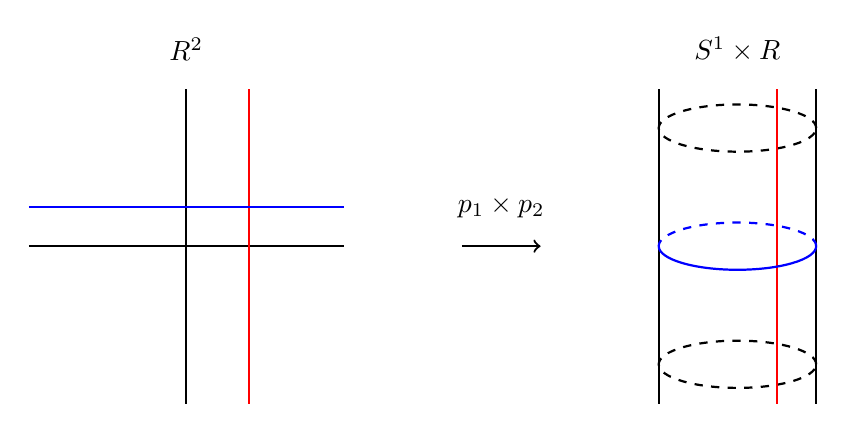
\begin{tikzpicture}
                \shorthandoff{>}

                % Ejes
                \draw[thick] (-4,-2) -- (-4,2); 
                \draw[thick] (-6,0) -- (-2,0);
                \node at (-4,2.5) {$\bb{R}^2$};

                % Líneas 1
                \draw[thick, red] (-3.2,-2) -- (-3.2,2);
                \draw[thick, blue] (-6, 0.5) -- (-2,0.5);

                % Función p
                \draw[thick, ->] (-0.5,0) -- (0.5,0);
                \node at (0,0.5) {$p_1\times p_2$};

                % Cilindro
                \draw[thick] (2,-2) -- (2,2);
                \draw[thick] (4,-2) -- (4,2);

                \draw[dashed, thick] (3,1.5) ellipse (1 and 0.3);
                \draw[dashed, thick] (3,-1.5) ellipse (1 and 0.3);

                \node at (3, 2.5) {$\bb{S}^1\times \bb{R}$};

                % Líneas 2
                \draw[thick, red] (3.5,-2) -- (3.5,2);

                \draw[blue, thick] (4,0) arc (0:-180:1 and 0.3);
                \draw[blue, dashed, thick] (4,0) arc (0:180:1 and 0.3);
                

            \end{tikzpicture}%
        \end{figure}%

        \item $\bb{R}^2$ es un recubridor del toro $\bb{S}^1\times \bb{S}^1$ de $\bb{R}^4$ (o el toro de rotación de $\bb{R}^3$ porque ambos toros son homeomorfos). Para ello consideramos 
        \begin{align*}
            p :\bb{R} & \to \bb{S}^1\\
            x & \mapsto (\cos(2\pi x), \sen(2\pi x))
        \end{align*}
         y su producto 
         \begin{align*}
            p\times p :\bb{R}\times \bb{R} & \to \bb{S}^1 \times \bb{S}^1\\
            x & \mapsto (\cos(2\pi x), \sen(2\pi x), \cos(2\pi x), \sen(2\pi x))
        \end{align*}
        que sería la aplicación recubridora. Intuitivamente podemos entenderlo de forma gráfica como \\

        \begin{figure}[H]
            \centering
            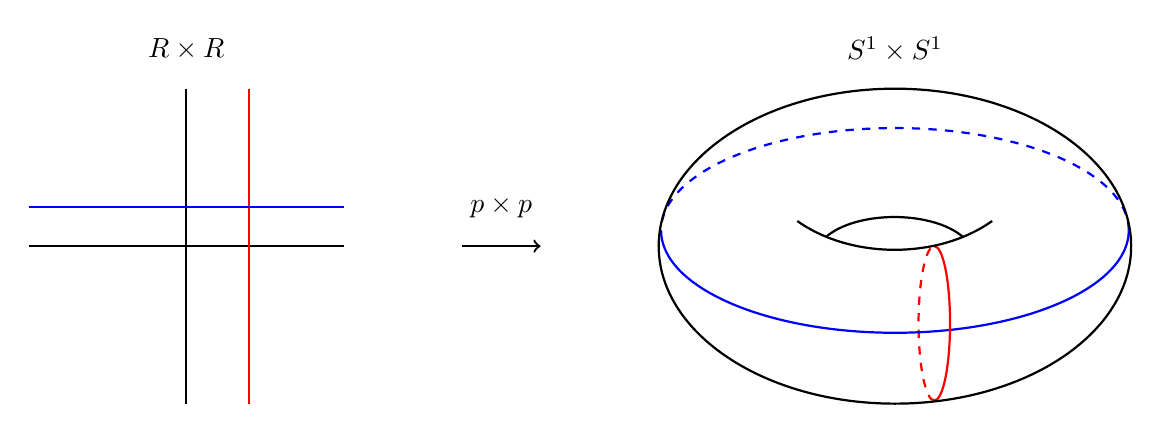
\begin{tikzpicture}
                \shorthandoff{>}

                % Ejes
                \draw[thick] (-4,-2) -- (-4,2); 
                \draw[thick] (-6,0) -- (-2,0);
                \node at (-4,2.5) {$\bb{R}\times \bb{R}$};

                % Líneas 1
                \draw[thick, red] (-3.2,-2) -- (-3.2,2);
                \draw[thick, blue] (-6, 0.5) -- (-2,0.5);

                % Función p
                \draw[thick, ->] (-0.5,0) -- (0.5,0);
                \node at (0,0.5) {$p\times p$};

                % Líneas 2
                \draw[thick, blue, dashed] (7.97,0.2) arc (0:180:2.97 and 1.3);
                \draw[thick, red, dashed] (5.5, -1.96) arc (-90:-270:0.2 and 0.98);
                \draw[thick, blue] (7.97,0.2) arc (0:-180:2.97 and 1.3);
                \draw[thick, red] (5.5, -1.96) arc (-90:90:0.2 and 0.98);


                % Toro
                \draw[thick] (5,0) ellipse (3 and 2);
                \draw[thick] (3.76,0.32) arc (225:315:1.75 and 1.25);
                % \draw[blue] (5,1) ellipse (1.75 and 1.25);
                \draw[thick] (5.86,0.12) arc (30:150:1 and 0.5);
                % \draw[red] (5,-0.2) ellipse (1 and 0.5);

                % \draw[thick, blue] (7.9,0.5) arc (0:-360:2.8 and 2.25);

                % \draw[thick, blue] (5,0.2) ellipse (2.97 and 1.3);
                % \draw[thick, red] (5.5, -0.98) ellipse (0.2 and 0.98);

                \node at (5,2.5) {$\bb{S}^1 \times \bb{S}^1$};            

            \end{tikzpicture}%
        \end{figure}%

        \item Intiutivamente podemos pensar en un recubrimiento de una circunferencia tangente a una recta como una colección de rectas paralelas y atravesadas por una común, como aparece en la figura. De esta forma (tal cual está en el dibujo) al ``enrollar'' el eje $x$ de forma que hagamos coincidir todas las rectas rojas tendremos que la recta azul forma una circunferencia, que como originalmente solo tocaba en un punto a cada recta, resultará en la circunferencia tangente a la recta.
        
        \begin{figure}[H]
            \centering
            \begin{tikzpicture}
                \shorthandoff{>}

                % Ejes
                \draw[thick] (-4,-2) -- (-4,2); 
                \draw[thick] (-6,0) -- (-2,0);
                \node at (-4,2.5) {$\bb{R}^2$};

                % Líneas 1
                \draw[thick, red] (-5.2,-2) -- (-5.2,2);
                \draw[thick, red] (-4.2,-2) -- (-4.2,2);
                \draw[thick, red] (-3.2,-2) -- (-3.2,2);
                \draw[thick, red] (-2.2,-2) -- (-2.2,2);

                \draw[thick, blue] (-6, 0.5) -- (-2,0.5);

                % Función p
                \draw[thick, ->] (-0.5,0) -- (0.5,0);
                \node at (0,0.5) {$p$};

                % Líneas 2
                \draw[thick, red] (2,-1.5) -- (8,-1.5);

                \draw[blue, thick] (5,0) circle [radius=1.5];


            \end{tikzpicture}%
        \end{figure}%
            
        \item Por último podemos plantearnos cómo podría ser un recubrimiento de dos circunferencias tangentes. Para ello, tal como aparece en la figura podremos usar una \textbf{cuadrícula}. De forma análoga al ejemplo anterior podremos ``enrollar'' en primer lugar el eje $x$ y obtendremos una única recta roja tangente a infinitas circunferencias azules (como en el ejemplo anterior pero con las circunferencias azules periódicas). Ahora podremos ``enrollar'' la propia recta roja, haciendo coincidir todas las circunferencias azules de forma que obtendremos las dos circunferencias tangentes.
        
        \begin{figure}[H]
            \centering
            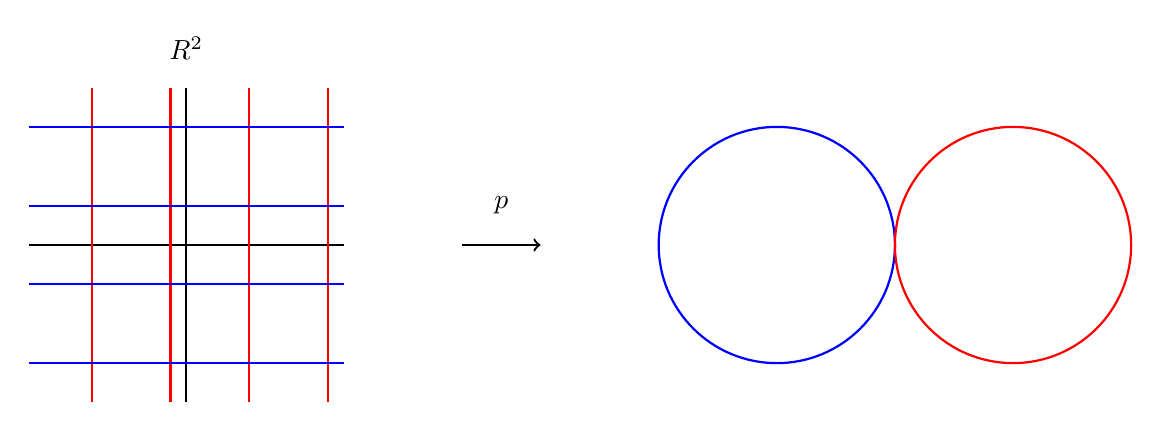
\begin{tikzpicture}
                \shorthandoff{>}

                % Ejes
                \draw[thick] (-4,-2) -- (-4,2); 
                \draw[thick] (-6,0) -- (-2,0);
                \node at (-4,2.5) {$\bb{R}^2$};

                % Líneas 1
                \draw[thick, red] (-5.2,-2) -- (-5.2,2);
                \draw[thick, red] (-4.2,-2) -- (-4.2,2);
                \draw[thick, red] (-3.2,-2) -- (-3.2,2);
                \draw[thick, red] (-2.2,-2) -- (-2.2,2);

                \draw[thick, blue] (-6, -1.5) -- (-2,-1.5);
                \draw[thick, blue] (-6, -0.5) -- (-2,-0.5);
                \draw[thick, blue] (-6, 0.5) -- (-2,0.5);
                \draw[thick, blue] (-6, 1.5) -- (-2,1.5);

                % Función p
                \draw[thick, ->] (-0.5,0) -- (0.5,0);
                \node at (0,0.5) {$p$};

                % Líneas 2
                \draw[blue, thick] (3.5,0) circle [radius=1.5];
                \draw[red, thick] (6.5,0) circle [radius=1.5];


            \end{tikzpicture}%
        \end{figure}%
    \end{enumerate}
\end{ejemplo}

\section{Levantamientos en espacios recubridores}

\begin{definicion}
    Sean $p:R\to B$ una aplicación recubridora y $f:X\to B$ una aplicación continua. Decimos que $\hat{f}:X\to R$ es un \textbf{levantamiento} de $f$ si se cumple que $\hat{f}$ es continua y $p\circ \hat{f} = f$. 
\end{definicion}

\begin{ejemplo}
    Consideramos la aplicación recubridora
    \begin{align*}
        p:\bb{R} & \to \bb{S}^1\\
        x & \mapsto (\cos(2\pi x), \sen(2\pi x))
    \end{align*}
    y tomamos
    \begin{align*}
        \alpha: [0,1] & \to \bb{S}^1\\
        s & \mapsto (\cos(2\pi s), \sen(2\pi s))
    \end{align*}
    Si elegimos
    \begin{align*}
        \hat{\alpha} : [0,1] \to \bb{R}\\
        s & \mapsto s
    \end{align*}
    es claro que $p\circ \hat{\alpha} = \alpha$. Otros posibles levantamientos de $\alpha$ son 
    \begin{align*}
        \hat{\alpha}_k : [0,1] & \to \bb{R}\ \ \ \ , k\in \bb{Z}  \\
        s & \mapsto k+s
    \end{align*}
    
    Nos planteamos ahora cuál sería un levantamiento de $\tilde{\alpha}(s) = \alpha(1-s)$. Podemos ver que $\hat{\tilde{\alpha}}_k(s) = k-s$ para $k\in \bb{Z}$ es en efecto un levantamiento de $\tilde{\alpha}(s)$.\\

    [Terminar Gráfica]

    \begin{figure}[H]
        \centering
        \begin{tikzpicture}
            \shorthandoff{>}

            % Ejes
            \draw[thick] (-4,-2) -- (-4,2); 
            \draw[thick] (-6,0) -- (-2,0);
            \node at (-4,2.5) {$\bb{R}^2$};

            % Líneas 1
            \node[draw, circle, fill=black, inner sep=1pt] at (-3.5,-0.25) {};
            \node[draw, circle, fill=black, inner sep=1pt] at (-2.25, 0.5) {};
            \draw[blue] plot[smooth, tension=1] coordinates {
                (-3.5,-0.25) (-3.25,0) (-3,0.75) (-2.5,0.6) (-2.25, 0.5)
            };

            % Función p
            \draw[thick, ->] (-0.5,0) -- (0.5,0);
            \node at (0,0.5) {$p$};

            % Cilindro
            \draw[thick] (2,-2) -- (2,2);
            \draw[thick] (4,-2) -- (4,2);

            \draw[dashed, thick] (3,1.5) ellipse (1 and 0.3);
            \draw[dashed, thick] (3,-1.5) ellipse (1 and 0.3);

            \node at (3, 2.5) {$\bb{S}^1\times \bb{R}$};

            % Líneas 2
            \draw[blue, thick] (4,0) arc (0:-180:1 and 0.3);
            \draw[blue, dashed, thick] (4,0) arc (0:180:1 and 0.3);
            \node[draw, circle, blue, fill=blue, inner sep=1pt, label=below:{$\alpha$}] at (3, -0.3) {};
            

        \end{tikzpicture}%
    \end{figure}%

\end{ejemplo}

\begin{lema}
    Sean $p:R\to B$ una aplicación recubridora, $r_0\in R$ y $b_0\in B$ tales que $p(r_0)=b_0$. Entonces dado un arco $\alpha:[0,1]\to B$ con $\alpha(0)=b_0$, existe un único arco $\hat{\alpha};[0,1]\to R$ tal que $\hat{\alpha}(0) = r_0$ y $\hat{\alpha}$ es un levantamiento de $\alpha$.

    \begin{proof}
        Como $p$ es una aplicación recubridora, cada punto $b\in B$ tiene asociado un abierto $O_b$ regularmente recubierto que contiene a $b$. Como $\alpha([0,1])$ es compacto tenemos que existe un recubrimiento finito, es decir,
        \begin{gather*}
            \alpha([0,1]) \subseteq O_{b_1} \cup O_{b_2}\cup \dots \cup O_{b_n}
        \end{gather*}
        Entonces $[0,1]\subseteq \alpha^{-1}( O_{b_1}) \cup \alpha^{-1}(O_{b_2})\cup \dots \cup \alpha^{-1}(O_{b_n})$ por lo que tendremos el intervalo $[0,1]$ recubierto por una familia finita de abiertos. Por el lema del número de Lebesgue\footnote{visto probablemente en alguna asignatura de Análisis.} sabemos que existe un $\delta>0$ tal que para cada $x\in[0,1]$ se tiene que $B(x,\delta)\cap[0,1]$ está contenido en algún $p^{-1}(O_{b_j})$ para cierto $j\in\{1,\dots,k\}$. Esto nos asegura que podemos hacer una subdivisión del intervalo $[0,1]$ tal que
        \begin{gather*}
            0 = t_0 < t_1 < \dots < t_{r-1} < t_r = 1
        \end{gather*}
        tal que $\alpha([t_j, t_{j+1}])$ está contenido en algún $O_{b_l}$ para $j\in\{0,\dots,r-1\}$, $l\in\{1,\dots,k\}$.

        Definimos $\hat{\alpha}$ de manera recursiva:\\

       $ \alpha([t_0,t_1])$ está contenido en algún $O_{b_l}$. Como $O_{b_l}$ está regularmente recubierto
       \begin{gather*}
            p^{-1}(O_{b_l}) = \bigcup\limits_{i\in I} A_i\ \ \text{ unión disjunta de abiertos}\\
            p_{|A_i}: A_i \to O_{b_l} \text{ es homeomorfismo}
       \end{gather*}

       Como $r_0\in p^{-1}(b_0) = p^{-1}(\alpha(0)) \subseteq p^{-1}(O_{b_l}) = \bigcup\limits_{i\in I}A_i$ se tiene que $r_0\in A_{i_0}$ para algún $A_{i_0}$ con $i_0\in I$. Como además $p_{|A_{i_0}}:A_{i_0} \to O_{b_l}$ es un homeomorfismo, podemos definir
       \begin{gather*}
            \hat{\alpha}(t) = (p_{|A_{i_0}})^{-1}(\alpha(t)),\ \ \ t\in [0=t_0, t_1]
       \end{gather*}
       Es claro que $\hat{\alpha}$ en $[0,t_1]$ es continua y $p\circ\hat{\alpha}=\alpha$.\\

       Para definir $\hat{\alpha}$ en $[t_1,t_2]$ repetimos el mismo procedimiento. Sabemos que $\alpha([t_1,t_2])$ cae en un abierto $O_{b_m}$ que está regularmente recubierto.
       \begin{gather*}
            p^{-1}(O_{b_m}) = \bigcup\limits_{i\in I'} A'_i\ \ \ \text{ con $A'_i$ abiertos disjuntos}\\
            p_{|A'_i} : A'_i \to O_{b_m} \text{ homeomorfismo}
       \end{gather*}
       Además tenemos que $\alpha(t_1)\in O_{b_m}$. Como $p(\hat{\alpha}(t_1)) = \alpha(t_1)\in O_{b_m}$, entonces $\hat{\alpha}(t_1)\in p^{-1}(O_{b_m})$ y por tanto $\exists i'_0$ tal que $\hat{\alpha}(t_1)\in A'_{i'_0}$. Como $p_{|A'_{i'_0}}:A'_{i'_0}:O_{b_m}$ es un homeomorfismo, podemos definir $\hat{\alpha}$ en $[t_1,t_2]$ como 
       \begin{gather*}
            \hat{\alpha}(t) = (p_{|A'_{i'_0}})^{-1}(\alpha(t))    
       \end{gather*}
       que es claramente contina y $(p\circ \hat{\alpha})(t)=\alpha(t)$ para $t\in [t_1,t_2]$. Por el lema de pegado tenemos que $\hat{\alpha}$ es continua en $[t_0,t_2]$. Siguiendo este procedimiento con cada $t_i$, $i\in\{0,\dots,r-1\}$ tendremos el resultado que buscábamos probar.\\

       Veamos ahora por qué $\hat{\alpha}$ es única con $\hat{\alpha}(0)=r_0$. Si existiese otro arco $\alpha^*:[0,1]\to R$ tal que $p\circ \hat{\alpha} = p\circ \alpha^*$ con $\hat{\alpha}(0) = r_0 = \alpha^*(0)$, entonces 
       \begin{gather*}
            \alpha([0=t_0,t_1]) \subset O_{b_l}
       \end{gather*}
       por lo que 
       \begin{gather*}
            \alpha^*([0,t_1]) \subseteq p^{-1}(O_{b_l}) = \bigcup\limits_{i\in I} A_i\\
            \hat{\alpha}([0,t_1]) \subseteq p^{-1}(O_{b_l}) = \bigcup\limits_{i\in I} A_i
       \end{gather*}
       Por continuidad, $\alpha^*([0,t_1])\subseteq A_{i_1}$ y $\hat{\alpha}([0,t_1])\subseteq A_{i_0}$ pero $\alpha^*(0)=r_0=\hat{\alpha}(0)\in A_{i_0}$ y como los $A_i$ son disjuntos tenemos que $A_{i_1} = A_{i_0}$. Además, $p_{|A_{i_0}}$ es homeomorfismo de $A_{i_0}$ en $O_{b_l}$ por lo que 
       \begin{gather*}
            \alpha^*(t) = \hat{\alpha}(t),\ \ \ t\in [0,1]
       \end{gather*}
       De forma recursiva se verifica la unicidad en todos los intervalos $[t_j, t_{j+1}]$ con $j\in \{0,\dots,r-1\}$.
    \end{proof}
\end{lema}

\begin{observacion}
    Es importante tener en cuenta que en general el levantamiento de un lazo no es un lazo, sino simplemente un arco.\\
\end{observacion}

\begin{lema}
    Sean $p:R \to B$ una aplicación recubridora y $H:[0,1]\times[0,1]\to B$ una aplicación continua. Dados $b_0=H(0,0)$ y $r_0\in p^{-1}(b_0)$, entonces existe un único levantamiento $\hat{H}:[0,1]\times[0,1]\to R$ tal que $\hat{H}(0,0) = r_0$. Si además $H$ es una homotopía por arcos, entonces $\hat{H}$ también lo será.
\end{lema}

\begin{coro}
    Sea $p:R\to B$ una aplicación recubridora, $\alpha$, $\beta:[0,1]\to B$ dos arcos con $[\alpha]=[\beta]$ y tomamos un $r_0\in p^{-1}(\alpha(0))$ ($\alpha(0)=\beta(0)$). Si elegimos $\hat{\alpha}, \hat{\beta}:[0,1]\to R$ como los únicos arcos con $\hat{\alpha}(0)=r_0=\hat{\beta}(0)$, entonces $[\hat{\alpha}] = [\hat{\beta}]$.
\end{coro}

\begin{definicion}
    Consideramos una aplicación recubridora $p:R\to B$, un punto $b_0\in B$ y otro $r_0\in R$ tal que $p(r_0)=b_0$. Entonces podemos definir la siguiente aplicación
    \begin{align*}
        \phi : \pi_1(B,b_0) & \to p^{-1}(b_0)\\
        [\alpha] & \mapsto \hat{\alpha}(1)
    \end{align*}
    donde $\hat{\alpha}$ es el único levantamiento de $\alpha$ con $\hat{\alpha}(0)=r_0$.
    % Lo importante de esta aplicación es que cuenta el número de vueltas de cada [\alpha].
    A la aplicación $\phi$ la llamaremos \textbf{correspondencia del levantamiento}.
\end{definicion}

\begin{ejemplo}
    Consideramos el caso de ``enrollar'' $\bb{R}$ sobre una circunferencia. La aplicación $\phi$ cuenta el número de vueltas que da cada arco, como se puede ver en el siguiente dibujo.
    \begin{figure}[H]
        \centering
        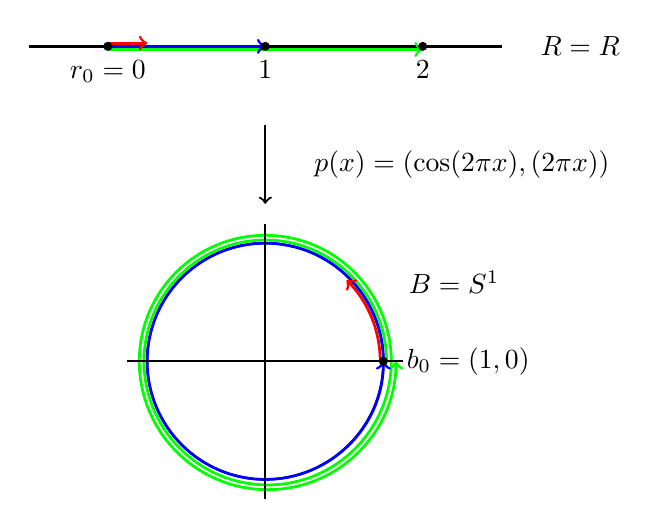
\begin{tikzpicture}
            \shorthandoff{>}

            % Recta
            \draw[line width=1pt] (-3,3) -- (3,3);
            \node at (4,3) {$R = \bb{R}$};

            % Abiertos en preimagen
            \draw[line width=1pt, green, ->] (-2, 2.96) -- (2, 2.96);
            \draw[line width=1pt, blue, ->] (-2, 3) -- (0, 3);
            \draw[line width=1pt, red, ->] (-2, 3.04) -- (-1.5, 3.04);

            % Puntos
            \node[draw, circle, fill=black, inner sep=1pt, label=below:{$r_0=0$}] at (-2,3) {};
            \node[draw, circle, fill=black, inner sep=1pt, label=below:$1$] at (0,3) {};
            \node[draw, circle, fill=black, inner sep=1pt, label=below:$2$] at (2,3) {};

            % Flecha función
            \draw[line width=0.8pt,->] (0,2) -- (0,1);
            \node[anchor=west] at (0.5,1.5) {$p(x) = (\cos(2\pi x), \sen(2\pi x))$};

            % Circunferencia
            \draw[thick] (0,-1) circle [radius=1.5];
            \node[anchor=west] at (1.7,0) {$B=\bb{S}^1$};
            \draw[green, line width=1pt] (1.54,-1) arc (0:180:1.54);
            \draw[green, line width=1pt] (1.6,-1) arc (0:-180:1.57);
            \draw[green, line width=1pt] (1.6,-1) arc (0:180:1.6);
            \draw[green, line width=1pt, <-] (1.66,-1) arc (0:-180:1.63);

            \draw[blue, line width=1pt, ->] (1.5,-1) arc (0:360:1.5);
            \draw[red, line width=1pt, ->] (1.46,-1) arc (0:45:1.46);
            
            \node[draw, circle, fill=black, inner sep=1pt, label=right:{\ $b_0 = (1,0)$}] at (1.5,-1) {};

            % Ejes
            \draw[thick] (0,-2.75) -- (0,0.75);
            \draw[thick] (-1.75,-1) -- (1.75,-1);

        \end{tikzpicture}%
    \end{figure}%
\end{ejemplo}

\begin{teo}
    Sean $p:R \to B$ una aplicación recubridora, $b_0\in B$, $r_0\in R$ con $p(r_0)=b_0$. Si $R$ es arcoconexo, entonces la correspondencia del levantamiento 
    \begin{align*}
        \phi: \pi_1(B,b_0) \to p^{-1}(b_0)
    \end{align*}
    es sobreyectiva. Además, si $R$ es simplemente conexo, entonces $\phi$ es biyectiva.
    \begin{proof}
        Si $R$ es arcoconexo tenemos que probar que dado $r_1\in p^{-1}(b_0)\subseteq R$ existe un lazo $\alpha:[0,1]\to B$ de forma que $\phi([\alpha]) = r_1$, es decir, su único levantamiento $\hat{\alpha}:[0,1]\to R$ cumple que $\hat{\alpha}(0) = r_0$ y $\hat{\alpha}(1) = r_1$.\\

        Para ello tomo un arco cualquiera $\alpha^*:[0,1]\to R$ tal que $\alpha^*(0) = r_0$ y $\alpha^*(1) = r_1$ que existe por ser $R$ arcoconexo. Elijo ahora $\alpha = p\circ \alpha^*$ que es un arco en $B$ tal que $\alpha(0)= p(\alpha^*(0)) = p(r_0) = b_0$ y $\alpha(1) = p(\alpha^*(1)) = p(r_1) = b_0$. Tenemos entonces que $\alpha$ es un lazo basado en $b_0$ y como $\alpha=p\circ \alpha^*$, entonces $\hat{\alpha} = \alpha^*$ es un levantamiento de $\alpha$ con $\hat{\alpha}(0) = \alpha^*(0) = r_0$ por lo que $\phi([\alpha]) = \hat{\alpha}(1) = \alpha^*(1) = r_1$.\\

        Nos queda ver que si $R$ es simplemente conexo, entonces $\phi$ es biyectiva. Como todo simplemente conexo es necesariamente arcoconexo sabemos de la primera parte del teorema que $\phi$ es sobreyectiva por lo que solo tenemos que probar la inyectividad. Eso es equivalente a considerar $[\alpha],[\beta]\in \pi_1(B,b_0)$ y ver si se verifica la implicación
        \begin{gather*}
             \phi([\alpha]) = \phi([\beta]) \overset{?}{\Rightarrow} [\alpha]=[\beta]
        \end{gather*}
        Sabiendo que $\hat{\alpha}(1) = \phi([\alpha])$ y $\hat{\beta}(1) = \phi([\beta])$. Como $\hat{\alpha}(1)=\hat{\beta}(1)$ consideramos $\hat{\alpha} \ast \hat{\beta}$ que es un lazo basado en $r_0$. Como $R$ es simplemente conexo tenemos que
        \begin{gather*}
            [\hat{\alpha}] \ast [\hat{\beta}] = [\hat{\alpha} \ast \hat{\beta}] = [\veps_{r_0}]
        \end{gather*}
        por lo que se tiene 
        \begin{gather*}
            [\hat{\alpha}] = [\veps_{r_0}] \ast [\hat{\beta}] = [\hat{\beta}]
        \end{gather*}
        Usando $p_*$ tenemos que
        \begin{gather*}
            p_*([\hat{\alpha}]) = [p\circ \hat{\alpha}] = [\alpha]\\
            p_*([\hat{\beta}]) = [p\circ \hat{\beta}] = [\beta]
        \end{gather*}
        y como $p_*([\hat{\alpha}]) = p_*([\hat{\beta}])$ llegamos a que $[\alpha] = [\beta]$ como queríamos demostrar.
    \end{proof}
\end{teo}

\section{Grupo fundamental de la circuferencia}

\begin{definicion}
    Dado un lazo $\alpha:[0,1]\to \bb{S}^1 \subseteq \bb{R}^2$ basado en $(1,0)$, definimos el grado de $\alpha$ como el único número entero $\hat{\alpha}(1)$ dado por el levantamiento $\hat{\alpha}$ de $\alpha$ mediante la aplicación recubridora
    \begin{gather*}
        p(x) = (\cos(2\pi x), \sen(2\pi x))\ \ \ \ , \text{con }\hat{\alpha}(0) \neq 0
    \end{gather*}
    Notaremos al grado de $\alpha$ como $\deg(\alpha)$
\end{definicion}

\begin{observacion}
    Como el grado es simplemente la correspondencia del levantamiento para $p$ y $r_0=0$, entonces si $[\alpha]=[\beta]$ se tiene que $\deg(\alpha)=\deg(\beta)$, es decir el grado está bien definido para clases de equivalencia.
\end{observacion}

\begin{teo}
    El grupo fundamental de $\bb{S}^1$ en el $(1,0)$ es isomorfo al grupo aditivo $(\bb{Z}, +)$. De hecho, la aplicación
    \begin{align*}
        \deg: \pi_1(\bb{S}^1, (1,0)) &\to \bb{Z}\\
        [\alpha] & \mapsto \deg(\alpha)
    \end{align*}
    es un isomorfismo de grupos.

    \begin{proof}
        Como $\bb{R}$ es simplemente conexo, el teorema anterior nos dice que  la aplicación $\deg$ es biyectiva. Tendremos que probar que $\deg$ es un homomorfismo, es decir que se verifica
        \begin{gather*}
            \deg([\alpha] \ast [\beta]) = \deg([\alpha]) + \deg([\beta])
        \end{gather*}
        Para verlo tomamos $\hat{\alpha}$, $\hat{\beta}$ levantamientos de $\alpha$ y $\beta$ respectivamente con 
        \begin{gather*}
            \hat{\alpha}(0) = 0 = \hat{\beta}(0)
        \end{gather*}
        Recordemos que $[\alpha] \ast [\beta] = [\alpha \ast \beta]$. Vamos a considerar
        \begin{gather*}
            \widehat{\alpha \ast \beta}(s) = \left\{
                \begin{array}{l c c}
                    \hat{\alpha}(2s) & \text{ si } & 0 \leq s \leq \nicefrac{1}{2}\\
                    \hat{\alpha}(1) + \hat{\beta}(2s-1) & \text{ si } &\nicefrac{1}{2} \leq s \leq 1
                \end{array}
            \right.
        \end{gather*}
        y es claro que $\widehat{\alpha \ast \beta}$ es continua. Queremos ver que $p(\widehat{\alpha\ast \beta}) = \alpha \ast \beta$. Desarrollando tenemos 
        \begin{align*}
            p(\widehat{\alpha \ast \beta})(s) &= \left\{
                \begin{array}{l c c}
                    p(\hat{\alpha}(2s)) & \text{ si } & 0 \leq s \leq \nicefrac{1}{2}\\
                    p(\hat{\alpha}(1) + \hat{\beta}(2s-1)) & \text{ si } &\nicefrac{1}{2} \leq s \leq 1
                \end{array}
            \right.\\\\
            &= \left\{
                \begin{array}{l c c}
                    \alpha(2s) & \text{ si } & 0 \leq s \leq \nicefrac{1}{2}\\
                    p(\hat{\beta}(2s-1)) & \text{ si } &\nicefrac{1}{2} \leq s \leq 1
                \end{array}
            \right\} = (\alpha \ast \beta)
        \end{align*}
        por lo que $\hat{\alpha\ast\beta}$ es un levantamiento de $\alpha \ast \beta$ con $\hat{\alpha \ast \beta}(0) = \hat{\alpha}(0)$ por lo que por definición tenemos que 
        \begin{gather*}
            \deg(\alpha \ast \beta) = \widehat{\alpha \ast \beta}(1) = \hat{\alpha}(1) + \hat{\beta}(1) = \deg(\alpha) + \deg(\beta)
        \end{gather*}
    \end{proof}
\end{teo}

\begin{observacion}
    Algunas consecuencias elementales son las siguientes
    \begin{itemize}
        \item El grupo fundamental de $\bb{S}^1\times \bb{R}$ es $\bb{Z}$. De aquí se deduce que $\bb{R}^2 \setminus \{p_0\}$ no es homeomorfo a $\bb{R}^2$ ya que $\bb{R}^2 \setminus \{p_0\}$ es homeomorfo a $\bb{S}^1\times \bb{R}$ que tiene por grupo fundamental $\bb{Z}$ y $\bb{R}^2$ tiene por grupo elemental el trivial.
        
        \item $\bb{R}^3\setminus R$ es homeomorfo a $(\bb{R}^2 \setminus \{(0,0)\}) \times \bb{R}$ donde $R$ es una recta en $\bb{R}^3$.
        
        \item El grupo fundamental del toro $\bb{S}^1 \times \bb{S}^1$ o el toro de rotación de $\bb{R}^3$ es $\bb{Z}\times \bb{Z}$.
    \end{itemize}
\end{observacion}

\begin{prop}\label{prop1-12}
    No existe ninguna aplicación continua\footnote{$\overline{\bb{D}}$ denota el disco cerrado de $\bb{R}^2$ centrado en el $(0,0)$ y con radio 1} $f : \overline{\bb{D}} \to \bb{S}^1$ tal que $f(x) = x$ para todo $x\in \bb{S}^1$

    \begin{proof}
        Tomamos $\alpha (s) = (\cos(2\pi s), \sen(2\pi s))$, lazo basado en $(1,0)$. Su clase de equivalencia en el disco sería 
        \begin{gather*}
            [\alpha]_{\overline{\bb{D}}} = [\veps_{(1,0)}]
        \end{gather*}
        ya que $\overline{\bb{D}}$ es simplemente conexo. Si exisitiese una $f$ continua, entonces tendríamos que
        \begin{align*}
            f_*:\pi_1(\overline{\bb{D}}(1,0)) & \to \pi_1(\bb{S}^1, (1,0))\text{ es homeomorfismo}\\
            [\alpha]_{\overline{\bb{D}}} & \mapsto f_*([\alpha]_{\overline{\bb{D}}}) \overset{def}{=}[f\circ \alpha]_{\bb{S}^1} = [\alpha]_{\bb{S}^1}
        \end{align*}
        Pero $[\alpha]_{\overline{\bb{D}}} = [\veps_{(1,0)}]$ por lo que 
        \begin{gather*}
            f_x([\alpha]_{\overline{\bb{D}}}) = f_*([\veps_{(1,0)}]_{\overline{\bb{D}}}) = [\veps_(1,0)]_{\bb{S}^1}
        \end{gather*}
        pero como $f_x([\alpha]_{\overline{\bb{D}}}) = [\alpha]_{\bb{S}^1}$ llegamos a contradicción ya que $\deg(\alpha) = 1$ y $\deg(\veps_{(1,0)}) = 0$
    \end{proof}
\end{prop}

\begin{teo}[punto fijo de Brouwer]
    Si $f:\overline{\bb{D}} \to \overline{\bb{D}}$ es continua, entonces existe $x_0\in \overline{\bb{D}}$ tal que $f(x_0)=x_0$.

    \begin{proof}
        Supongamos que $f$ no tiene ningún punto fijo, es decir, $f(x)\neq x$ para todo $x\in \overline{\bb{D}}$. Buscaremos ahora construir una aplicación a partir de esta hipótesis que deje a los puntos de la circunferencia $\bb{S}^1$ fijos para poder aplicar la proposición anterior. \\

        Para cada $x$ consideramos la semirrecta abierta 
        \begin{gather*}
            f(x) + \lambda_x (x-f(x))\ \ \ \forall \lambda_x >0
        \end{gather*}
        y la intersección de dicha semirrecta con la circunferencia unidad. Como $f(x),x\in \overline{\bb{D}}$ y $f(x)\neq x$, lo recién definido es efectivamente una semirrecta y ha de cortar exactamente en un único punto a $\bb{S}^1$.
        \begin{gather*}
            1 = \langle f(x) + \lambda_x (x-f(x)), f(x) + \lambda_x (x-f(x)) \rangle =\\
            \langle f(x) \rangle + 2\lambda_x \langle f(x), x-f(x)\rangle + \lambda_x^2 \langle x-f(x), x-f(x) \rangle
        \end{gather*}
        Por lo que podemos despejar $\lambda_x$ y nos queda
        \begin{gather*}
            \lambda_x = \frac{-2\langle f(x), x-f(x) \rangle + \sqrt{4\langle f(x), x-f(x)\rangle^2 - 4(\langle f(x),f(x)-1\rangle)\langle x-f(x), x-f(x)\rangle}}{2\langle x-f(x), x-f(x) \rangle}
        \end{gather*}
        Por lo que $g(x) = f(x) + \lambda_x(x-f(x))$ es continua y $|g(x)|=1$. Por tanto tenemos que si $x\in \bb{S}^1$, entonces $g(x)=x$ lo que contradice la proposición anterior.
    \end{proof}
\end{teo}

\begin{observacion}
    El teorema del punto fijo de Brouwer no solo es cierto para $\overline{\bb{D}}$ sino para cualquier espacio topológico $X$ homeomorfo a $\overline{\bb{D}}$. Es decir, si $f:X\to X$ es continua con $X$ homeomorfo a $\overline{\bb{D}}$, entonces existe al menos un punto $x_0\in X$ tal que $f(x_0)=x_0$.

    \begin{proof}
        Notemos por $h:\overline{\bb{D}}\to X$ al homeomorfismo y estaremos en la siguiente situación
        \begin{gather*}
            \overline{\bb{D}} \overset{h}{\longrightarrow} X \overset{f}{\longrightarrow} X \overset{h^{-1}}{\longrightarrow} \overline{\bb{D}}
        \end{gather*}
        Entonces tendríamos $h^{-1}\circ f \circ h : \overline{\bb{D}} \to \overline{\bb{D}}$ continua y por el teorema de Brower existe $y_0\in \overline{\bb{D}}$ tal que $(h^{-1}\circ f \circ h)(y_0) = y_0$.
    \end{proof}
\end{observacion}

\begin{coro}
    Sea $V:\overline{\bb{D}}\to \bb{R}^2 \setminus \{(0,0)\}$ una aplicación continua. Entonces existen puntos $x,y\in \bb{S}^1$ de forma que $V(x) = \lambda x$, $V(y) = -\mu y$ con $\lambda, \mu >0$.

    \begin{proof}
        Consideramos la aplicación $f(x) = \frac{V(x)}{|V(x)|}$ que es continua (ya que $V(x)\neq 0$ para todo $x\in \overline{{\bb{D}}}$). Por el teorema de Brouwer tenemos que $\exists x_0\in \overline{\bb{D}}$ tal que $f(x_0) = x_0$ por lo que $x_0 = \frac{V(x_0)}{|V(x_0)|}$ y entonces $V(x_0) = |V(x_0)|x_0 = \lambda x_0$ (tomando $\lambda = |V(x_0|$). Si tomamos $g(x) = - \frac{V(x_0)}{|V(x_0)|}$ tendríamos análogamente que existe un $y_0$ tal que $y_0 = g(y_0) = \frac{V(y_0)}{|V(y_0)|}\in \bb{S}^1$ y $V(y_0) = -|V(y_0)|y_0 = -\mu y_0$ (tomando $\mu = |V(y_0)|$). En general, para poder considerar cualquier ángulo $\theta$ tendremos que considerar
        \begin{gather*}
            h(x) = \frac{V(x)}{e^{i\theta} |V(x)|}
        \end{gather*}
    \end{proof}
\end{coro}

\begin{teo}[Teorema fundamental del álgebra]
    Todo polinomio complejo de grado $n \geq 1$ tiene al menos una raíz compleja
    \begin{proof}
        Vamos a considerar $p(z) = a_0+a_1z + \dots + a_{n-1}z^{n-1} + z^n$ con $n\geq 1$ y supongamos que $p(z)\neq 0$ \ $\forall z \in \bb{C}$, es decir, que no tiene raíces en $\bb{C}$. Consideramos la siguiente aplicación
        \begin{gather*}
            H(s,t) = \left\{
                \begin{array}{l c c}
                    \dfrac{p\left(\dfrac{t}{1-t} e^{2\pi i s}\right) \cdot \left|p\left(\dfrac{t}{1-t}\right)\right|}{\left|p\left(\dfrac{t}{1-t} e^{2\pi i s}\right)\right| \cdot p\left(\dfrac{t}{1-t}\right)} & \text{ si } & (s,t)\in [0,1]\times [0,1[\\\\
                    e^{2\pi i n s} & \text{ si } & (s,t)\in [0,1]\times\{1\}
                \end{array}
            \right.
        \end{gather*}
        Esta aplicación lo que hace es considerar el plano complejo y su imagen mediante $p$. La aplicación $p$ no pasa por el origen porque así lo hemos supuesto. Para $t=0$ (tiempo inicial) tenemos que $H(s,0) = (1,0)_{\bb{R}^2} \equiv 1_{\bb{C}}$. Además para $s=0$ tenemos $H(0,t) = (1,0)_{\bb{R}^2} \equiv 1_{\bb{C}}$. Si la aplicación $H$ fuera una homotopía, al principio (cuando $t$ es bajo) no daría ninguna vuelta (en la imagen) y al final (cuando domina $z^n$) daría $n$ vueltas por lo que no puede ser.\\

        Comprobemos que $H$ es continua. Para esto simplemente veamos que 
        \begin{gather*}
            \lim_{t\to 1^-}\frac{p\left(\frac{t}{1-t} e^{2\pi i s_0}\right) \cdot \left|p\left(\frac{t}{1-t}\right)\right|}{\left|p\left(\frac{t}{1-t} e^{2\pi i s_0}\right)\right| \cdot p\left(\frac{t}{1-t}\right)} = e^{2 \pi i n s_0}\\\\
            \lim_{t\to 1^-}\frac{p\left(\frac{t}{1-t} e^{2\pi i s_0}\right) \cdot \left|p\left(\frac{t}{1-t}\right)\right|}{\left|p\left(\frac{t}{1-t} e^{2\pi i s_0}\right)\right| \cdot p\left(\frac{t}{1-t}\right)} =\\
            = \lim_{t\to 1^-} \frac{\left(\left(\frac{t}{1-t}\right)^n e^{2\pi i n s_0} + a_{n-1} \left(\frac{t}{1-t}\right)^{n-1} e^{2\pi i (n-1) s_0} + \dots\right) \cdot \left|\left(\frac{t}{1-t}\right)^n + a_{n-1} \left(\frac{t}{1-t}\right)^{n-1}  + \dots\right|  }%
            {\left|\left(\frac{t}{1-t}\right)^n e^{2\pi i n s_0} + a_{n-1} \left(\frac{t}{1-t}\right)^n e^{2\pi i (n-1) s_0} + \dots\right| \cdot \left(\left(\frac{t}{1-t}\right)^n + a_{n-1} \left(\frac{t}{1-t}\right)^{n-1}  + \dots\right)} = \\
            = \frac{e^{2\pi i n s_0}}{|e^{2\pi i n s_0|}} \cdot \frac{|1|}{1} = e^{2\pi i n s_0}
        \end{gather*}
        y tenemos claramente que $H:[0,1]\times [0,1]\to \bb{S}^1$ es continua. Además se tiene 
        \begin{align*}
            H(0,t) = 1\ \ \ \ \ & t\in [0,1]\\
            H(1,t) = 1\ \ \ \ \  & t\in [0,1]\\
            H(s,0) = 1\ \ \ \ \  & s\in [0,1]\\
            H(s,1) = e^{2\pi i n s} \ \ \ \ \ & s\in [0,1]
        \end{align*}
        por lo que $H$ es una homotopía por arcos entre los lazos $\alpha_1(s) = 1$ y $\alpha_2(s) = e^{2\pi i n s}$. Entonces tendremos que 
        \begin{gather*}
            [\alpha_1] = [\alpha_2] \ \ \ \text{ y } \ \ \ 0 = \deg(\alpha_1) = \deg(\alpha_2) = n
        \end{gather*}
        y llegamos a contradicción ya que $n\geq 1$. Por tanto $\exists z \in \bb{C}$ tal que $f(z) = 0$.
    \end{proof}
\end{teo}

\section{Retracciones, tipos de homotopía y retractos de deformación}

\begin{definicion}
    Sea $X$ un espacio topológico y $A\subseteq X$. Decimos que una aplicación continua $r:X \to A$ es una \textbf{retracción} si se cumple que $r(a) = a\ \ \forall a \in A$.\\

    Se dice que $A$ es un \textbf{retracto} de $X$ si existe una retracción $r:X \to A$.
\end{definicion}

\begin{ejemplo}\
    \begin{enumerate}
        \item $\bb{S}^1$ es un retracto de $\bb{R}^{n+1}\setminus \{0\}$. Podemos considerar
        \begin{align*}
            r:\bb{R}^{n+1}\setminus \{0\} &\to \bb{S}^1\\
            x & \mapsto \frac{x}{|x|}
        \end{align*}
        que es claramente continua y $r(x) = x$ para todo $x\in \bb{S}^1$.

        \item $\bb{S}$ no es un retracto de $\overline{\bb{D}}$ por lo visto en la proposición \ref{prop1-12}.
        
        \item La compresión de un cuadrado también es un retracto. 
        \begin{figure}[H]
            \centering
            \begin{tikzpicture}[scale=0.8]
                \shorthandoff{>}

                % Ejes
                \draw[thick] (-3,-2) -- (-3,2);
                \draw[thick] (-5,-2) -- (-5,2);
                \draw[thick] (-6,1) -- (-2,1);
                \draw[thick] (-6,-1) -- (-2,-1);

                \node at (-4,2.5) {$X$};


                % Función p
                \draw[thick, ->] (-0.5,0) -- (0.5,0);
                \node at (0,0.5) {$r$};

                % Cuadrado
                \draw[thick] (2,-1) -- (2,1);
                \draw[thick] (4,-1) -- (4,1);
                \draw[thick] (2,-1) -- (4,-1);
                \draw[thick] (4,1) -- (2,1);

            \end{tikzpicture}
        \end{figure}
    \end{enumerate}
\end{ejemplo}

\begin{lema}
    Sean $X$ un e.t. y $A\subseteq X$ tal que $A$ es un retracto de $X$. Entonces la aplicación inclusión $i:A\to X$ induce un homomorfismo inyectivo
    \begin{gather*}
        i_* : \pi_1(A, a_0) \to \pi_1(X,a_0)
    \end{gather*}

    \begin{proof}
        Si $A$ es retracto de $X$, entonces por definición tenemos que  $\exists r :X \to A$ continua tal que $r(a)=a$ para cualquier $a\in A$.
        \begin{align*}
            A \overset{i}{\longrightarrow} X \overset{r}{\longrightarrow} A& \ \ \ ,r\circ i = Id_A\\
            a \longmapsto a  \longmapsto a&
        \end{align*}

        \begin{gather*}
            \xymatrix{
                \pi_1(A,a_0) \ar[r]^{i_*} \ar@/_1pc/[rr]_{r_* \circ i_*} &
                \pi_1(X,a_0) \ar[r]^{r_*} &
                \pi_1(A,a_0)
            }
        \end{gather*}

        \begin{gather*}
            r_* \circ i_* = (Id_a)_* = Id_{\pi_1(A,a_0)}
        \end{gather*}
            
        Como $Id_{\pi_1(A,a_0)}$ es inyectiva, entonces se tiene que $i_*$ es inyectiva.
    \end{proof}
\end{lema}

\begin{definicion}
    Sea $f:X\to Y$ una aplicación continua entre dos espacios topológicos. Decimos que $f$ es una \textbf{equivalencia homotópica} si existe $g:Y\to X$ continua tal que $g\circ f$ es homotópica a $Id_X$ y $f\circ g$ es homotópica a $Id_Y$.\\

    Decimos que $X$ e $Y$ son \textbf{homotópicamente equivalentes} si existe una equivalencia homotópica entre ambos.\\

    A la aplicación $g$ se le llama una \textbf{inversa homotópica} de $f$.
\end{definicion}

\begin{observacion}\
    \begin{enumerate}
        \item[(i)] La inversa homotópica no tiene por qué ser única
        \item[(ii)] La composición de equivalencias homotópicas sigue siendo una equivalencia homotópica, de lo que se deduce que ser homotópicamente equivalente es una relación de equivalencia.
        \item[(iii)] Una equivalencia homotópica no tiene por qué ser ni inyectiva ni sobreyectiva. 
        \item[(iv)] Todo heomorfismo es una equivalencia homotópica.
    \end{enumerate}
\end{observacion}

\begin{lema}
    Sean $f,g:X\to Y$ dos aplicaciones continuas, $x_0\in X$. Si $H$ es una homotopía entre $f$ y $g$ y consideramos el arco $\alpha(t)=H(x_0, t)$. Entonces se tiene que el siguiente diagrama es conmutativo
    \begin{gather*}    
        \xymatrix{ %
        & \pi_1(Y,f(x_0)) \ar[dd]^{\displaystyle\varphi \equiv \text{isomorfismo}}\\
        \pi_1(X,x_0) \ar[ur]^{\displaystyle f_*} \ar[dr]^{\displaystyle g_*}\\ 
        & \pi_1(Y, g(x_0))
        }
    \end{gather*}
    donde $\phi([\gamma]) = [\tilde{\alpha}] \ast [\gamma] \ast [\alpha]$. En particular, $f_*$ es inyectiva (respectivamente sobreyectiva) si y solo si $g_*$ lo es.

    \begin{proof}
        Tenemos que demostrar que si $\beta$ es un lazo en $X$ basado en $x_0$, entonces:
        \begin{gather*}
            (\varphi \circ f_*) ([\beta]) = g_*([\beta]) = [g\circ \beta]
        \end{gather*}
        Pero tenemos además
        \begin{gather*}
            (\varphi \circ f_*) ([\beta]) = [\tilde{\alpha}] \ast [f\circ \beta] \ast [\alpha]
        \end{gather*}
        por lo que será equivalente a probar que
        \begin{gather*}
            [\alpha]\ast [g\circ \beta] = [f\circ \beta] \ast [\alpha]
        \end{gather*}
        es decir, que existe una homotopía por arcos que lleva $\alpha \ast(g\circ \beta)$ en $(f\circ \beta) \ast \alpha$.\\

        \begin{figure}[H]
            \centering

            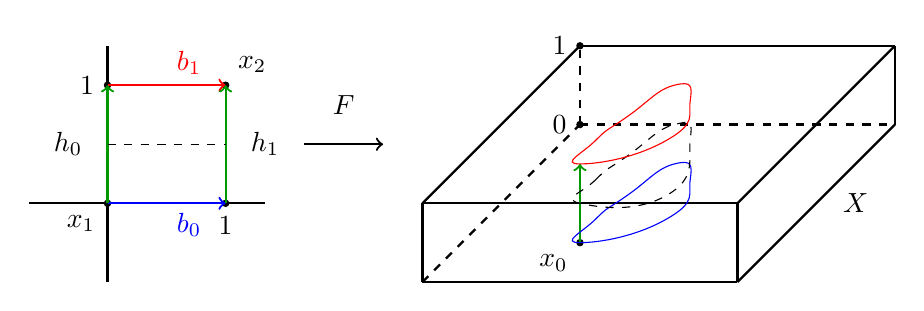
\begin{tikzpicture}
                % Aplicación F
                \node at (0,1.25) {$F$};
                \draw[thick,->] (-0.5,0.75) -- (0.5,0.75);


                % Ejes 1
                \draw[thick] (-3,-1) -- (-3,2);
                \draw[thick] (-4,0) -- (-1,0);

                \node[draw, circle, fill=black, inner sep=0.8pt, label=below left:{$x_1$}] at (-3,0) {};
                \node[draw, circle, fill=black, inner sep=0.8pt, label=below:{$1$}] at (-1.5,0) {};
                \node[draw, circle, fill=black, inner sep=0.8pt, label=left:{$1$}] at (-3,1.5) {};
                \node[draw, circle, fill=black, inner sep=0.8pt, label=above right:{$x_2$}] at (-1.5,1.5) {};

                % Cierre del cuadrado
                \draw[thick, ->, blue] (-3,0) -- node[below right] {$b_0$}(-1.5,0);
                \draw[thick, ->, red] (-3,1.5) -- node[above right] {$b_1$}(-1.5,1.5);

                \draw[thick, ->, green!60!black] (-1.5,0) -- (-1.5,1.5);
                \draw[thick, ->, green!60!black] (-3,0) -- (-3,1.5);

                \draw[dashed] (-3,0.75) -- (-1.5,0.75);
                \node at (-3.5, 0.75) {$h_0$};
                \node at (-1, 0.75) {$h_1$};
                

                % Caja
                \draw[thick, dashed] (3,1) -- (3,2);
                \draw[thick, dashed] (3,1) -- (7,1);
                \draw[thick] (7,1) -- (7,2);
                \draw[thick] (3,2) -- (7,2);
                \draw[thick] (1,-1) -- (1,0);
                \draw[thick] (1,-1) -- (5,-1);
                \draw[thick] (5,-1) -- (5,0);
                \draw[thick] (1,0) -- (5,0);
                \draw[thick, dashed] (1,-1) -- (3,1);
                \draw[thick] (1,0) -- (3,2);
                \draw[thick] (5,-1) -- (7,1);
                \draw[thick] (5,0) -- (7,2);

                % Puntos y leyenda
                \node[draw, circle, fill=black, inner sep=0.8pt, label=left:{$0$}] at (3,1) {};
                \node[draw, circle, fill=black, inner sep=0.8pt, label=left:{$1$}] at (3,2) {};
                \node at (6.5,0) {$X$};

                \node[draw, circle, fill=black, inner sep=0.8pt, label=below left:{$x_0$}] at (3,-0.5) {};
                \draw[thick, ->, green!60!black] (3,-0.5) -- (3,0.5);

                % Curva
                \draw[blue] plot[smooth cycle, tension=1] coordinates {
                    (3,-0.5) (3.2,-0.2) (3.6,0.1) (4.2,0.5) (4.4,0.3) (4.1,-0.2)
                };
                \draw[dashed] plot[smooth cycle, tension=1] coordinates {
                    (3,0) (3.2,0.3) (3.6,0.6) (4.2,1) (4.4,0.8) (4.1,0.1)
                };
                \draw[red] plot[smooth cycle, tension=1] coordinates {
                    (3,0.5) (3.2,0.8) (3.6,1.1) (4.2,1.5) (4.4,1.3) (4.1,0.8)
                };

            \end{tikzpicture}
        \end{figure}

        Por hipótesis tenemos $H:X\times[0,1]\to Y$ continua tal que 
        \begin{align*}
            &(x,0) \mapsto f(x)\\
            &(x,1) \mapsto g(x)\\
            &\alpha(t) = H(x_0,t)
        \end{align*}
        Definimos la siguiente aplicación
        \begin{align*}
            F:[0,1]\times [0,1] & \to X\times [0,1]\ \ \ \text{ continua}\\
            (s,t) & \mapsto (\beta(s), t)
        \end{align*}
        que verifica
        \begin{align*}
            b_0(s) = (s,0)\ \ \ \ \ & ,s\in [0,1]\\
            b_1(s) = (s,1)\ \ \ \ \  & ,s\in [0,1]\\
            h_0(s) = (0,s)\ \ \ \ \  & ,s\in [0,1]\\
            h_1(s) = (1,s)\ \ \ \ \ & ,s\in [0,1]
        \end{align*}
        Como $[0,1]\times [0,1]$ es simplemente conexo y $b_0\ast h_1 \ast \tilde{b_1} \ast \tilde{h_0}$ es un lazo en el $(0,0)$, entonces se tiene que 
        \begin{gather*}
            [b_0\ast h_1 \ast \tilde{b_1} \ast \tilde{h_0}] = [\veps_{(0,0)}] \Rightarrow [b_0\ast h_1] = [h_0\ast b_1]
        \end{gather*}
        Por tanto tenemos que $\exists G:[0,1]\times[0,1] \to [0,1]\times[0,1]$ homotopía por arcos tal que $G(s,0) = (b_0\ast h_1)(s)$ y $G(s,1) = (h_0\ast b_1)(s)$ por lo que quedan los extremos fijos, es decir, $G(0,t) = (0,0)$ y $G(1,t) = (1,1)$. Consideramos entonces
        \begin{gather*}
            H\circ F \circ G : [0,1] \times [0,1] \to Y\ \ \  \text{ continua}
        \end{gather*}
        y tenemos que 
        \begin{gather*}
            (H\circ F \circ G) (0,t) = H(F(0,0)) = H(x_0,0) = f(x_0)\\
            (H\circ F \circ G) (1,t) = H(F(1,1)) = H(x_0,1) = g(x_0)\\
            (H\circ F \circ G) (s,0) = H(F((b_0\ast h_1)(s))) = (H\circ F)\left(\left\{
                \begin{array}{l c c}
                    b_0(2s) & \text{ si } & s\in [0, \nicefrac{1}{2}]\\
                    h_1(2s-1) & \text{ si } & s \in [\nicefrac{1}{2}, 1]
                \end{array}
            \right\}\right) = \\
            = (H\circ F) \left(\left\{
                \begin{array}{l c c}
                    (2s,0) & \text{ si } & s\in [0, \nicefrac{1}{2}]\\
                    (1, 2s-1) & \text{ si } & s \in [\nicefrac{1}{2}, 1]
                \end{array}
            \right\}\right) =
            H \left(\left\{
                \begin{array}{l c c}
                    (\beta(2s), 0) & \text{ si } & s\in [0, \nicefrac{1}{2}]\\
                    (x_0, 2s-1) & \text{ si } & s \in [\nicefrac{1}{2}, 1]
                \end{array}
            \right\}\right) = \\
            = \left\{
                \begin{array}{l c c}
                    f(\beta(2s)) & \text{ si } & s\in [0, \nicefrac{1}{2}]\\
                    \alpha(2s-1) & \text{ si } & s \in [\nicefrac{1}{2}, 1]
                \end{array}
            \right\} = ((f\circ \beta) \circ \alpha)(s)
        \end{gather*}
        Análogamente se tiene que 
        \begin{gather*}
            (H\circ F \circ G) (s,1) = (\alpha \ast (g\circ \beta))(s)
        \end{gather*}
        Por lo que llegamos a que
        \begin{gather*}
            [\alpha]\ast [g\circ \beta] = [f\circ \beta] \ast [\alpha]
        \end{gather*}
        como queríamos probar.
    \end{proof}
\end{lema}

\begin{teo}
    Sea $f:X\to Y$ una equivalencia homotópica, entonces
    \begin{gather*}
        f_*: \pi_1(X,x_0)\to \pi_1(Y,f(x_0))
    \end{gather*}
    es un isomorfismo.
    \begin{proof}
        Como $f$ es una equivalencia homotópica, existe $g:Y\to X$ que es una inversa homotópica suya. Sabemos que $g\circ f$ es homotópica a $Id_X$ entonces:
        \begin{gather*}
            \xymatrix{ %
            \pi_1(X,x_0) \ar[r]^{(f_0)_*} \ar[drr]_{\overset{\scriptstyle(Id_X)_*}{\text{isom.}}} & \pi_1(Y,f(x_0)) \ar[r]^{g_*} & \pi_1(X,g(f(x_0))) \ar[d]^{\displaystyle \varphi \equiv \text{isomorfismo}}\\
            && \pi_1(X,x_0)
            \ar@{}[lu]|{//}
            }
        \end{gather*}
        De aquí se deduce que $(f_{x_0})_*$ es inyectiva y que $g_*$ es sobreyectiva
        \begin{gather*}
            \xymatrix{ %
            \pi_1(Y,f(x_0)) \ar[r]^{g_*} \ar[drrr]_{\overset{\scriptstyle(Id_Y)_*}{\text{isom.}}} & \pi_1(X,g(f(x_0))) \ar[rr]^{(f\circ g\circ f(x_0))_*} && \pi_1(Y, f(g(f(x_0)))) \ar[d]^{\displaystyle \tilde{\varphi} \equiv \text{isomorfismo}}\\
            &&& \pi_1(X,x_0)
            \ar@{}[lu]|{//}
            }
        \end{gather*}
    \end{proof}
\end{teo}

\begin{definicion}
    Sean $X$ un espacio topológico y $A\subset X$. Decimos que $A$ es un \textbf{retracto de deformación} de $X$ si existe una retracción $r:X\to A$ que es homotópica a la identidad en $X$.\\

    Esta definición se escribe simplemente como que existe $H:X\times[0,1]\to X$ homotopía tal que 
    \begin{gather*}
        H(x,0) = x \ \ \ \forall x \in X\\
        H(x,1) \in A \ \ \ \forall x \in X\\
        H(a,1) = a \ \ \ \forall a\in A\\
    \end{gather*}
    Aquí la retracción es simplemente $r(x)=H(x,1)$.
\end{definicion}

\begin{ejemplo}\
    \begin{enumerate}
        \item $X=\bb{S}^1 \cup (\bb{R}\times\{1\})$. 
        
        \begin{figure}[H]
            \centering
            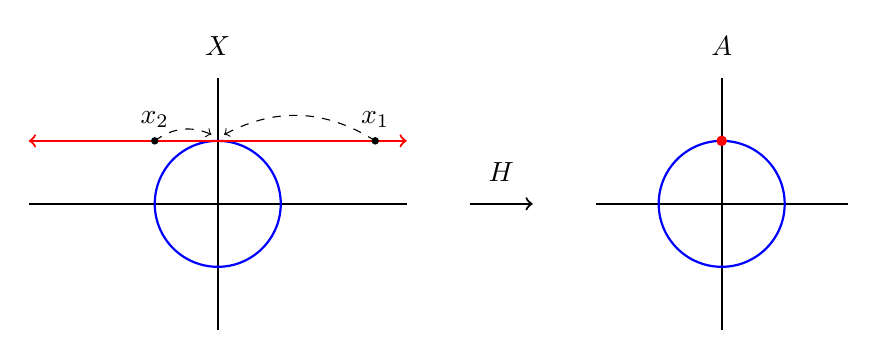
\begin{tikzpicture}[scale=0.8]
                \shorthandoff{>}

                % Ejes X
                \draw[thick] (-4,-2) -- (-4,2);
                \draw[thick] (-7,0) -- (-1,0);

                % Espacio X
                \draw[thick, blue] (-4,0) circle [radius=1];

                \draw[thick, red, <->] (-7,1) -- (-1,1);

                \node at (-4,2.5) {$X$};


                % Funciones de los puntos
                \draw[->, bend right=30, dashed] (-1.5, 1) to (-3.9,1.1) ;
                \node[draw, circle, fill=black, inner sep=0.8pt, label =above:{$x_1$}] at (-1.5,1) {};

                \draw[->, bend left=30, dashed] (-5, 1) to (-4.1,1.1) ;
                \node[draw, circle, fill=black, inner sep=0.8pt, label =above:{$x_2$}] at (-5,1) {};

                % Función H
                \draw[thick, ->] (0,0) -- (1,0);
                \node at (0.5,0.5) {$H$};

                % Ejes A
                \draw[thick] (4,-2) -- (4,2);
                \draw[thick] (6,0) -- (2,0);

                \node at (4,2.5) {$A$};

                % Círculo en A
                \draw[thick, blue] (4,0) circle [radius=1];

                \node[draw, circle, red, fill=red, inner sep=1.2pt] at (4,1) {};

                % Puntos A
                % \node[draw, circle, fill=black, inner sep=0.8pt, label =above left:{$1$}] at (4,1) {};
                

            \end{tikzpicture}
        \end{figure}
        
        Veamos que $\bb{S}^1$ es retracto de deformación de $X$. Para ello buscamos $H:X\times[0,1]\to X$ y la definimos de la siguiente forma:
        \begin{gather*}
            H(x,t) = \left\{
                \begin{array}{l c c }
                    x & \text{ si } & x\in \bb{S}^1,\ t\in [0,1]\\
                    (1-t)x+t(0,1) & \text{ si } & x\in \bb{R}\times\{1\},\ t\in [0,1]
                \end{array}
            \right.
        \end{gather*}
        Con esta definición tenemos
        \begin{align*}
            H(x,0) &= x \ \ \ \forall x \in X\\
            H(x,1) &=  \left\{
                \begin{array}{l c c }
                    x & \text{ si } & x\in \bb{S}^1\\
                    (0,1) & \text{ si } & x\in \bb{R}\times\{1\}
                \end{array}
            \right\} \Rightarrow H(x,1)\in \bb{S}^1 \ \ \ \forall x \in X\\
            H(a,0) &= a \ \ \ \forall a\in \bb{S}^1\\
        \end{align*}
        y tenemos la retracción definida como se ha hecho en la definición.

        \item $X=(\bb{R}\times \{-1,1\})\cup (\{-1,1\}\times \bb{R})$. 
        
        \begin{figure}[H]
            \centering
            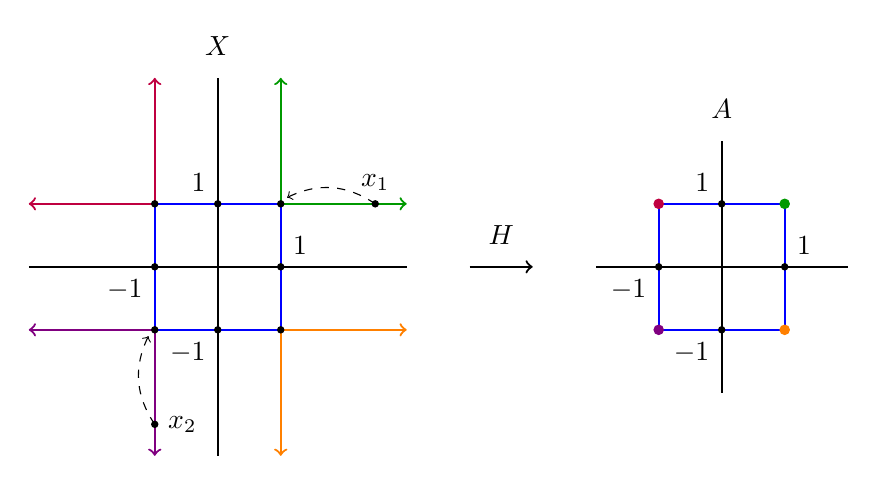
\begin{tikzpicture}[scale=0.8]
                \shorthandoff{>}

                % Ejes X
                \draw[thick] (-4,-3) -- (-4,3);
                \draw[thick] (-7,0) -- (-1,0);

                % Espacio X
                \draw[thick, purple, <->] (-5,3) -- (-5,1) -- (-7,1);
                \draw[thick, green!60!black, <->] (-3,3) -- (-3,1) -- (-1,1);
                \draw[thick, orange, <->] (-3,-3) -- (-3,-1) -- (-1,-1);
                \draw[thick, violet, <->] (-5,-3) -- (-5,-1) -- (-7,-1);

                \draw[thick, blue] (-5,1) -- (-3,1) -- (-3,-1) -- (-5,-1) -- cycle;

                \node at (-4,3.5) {$X$};

                % Puntos X
                \node[draw, circle, fill=black, inner sep=0.8pt] at (-5,1) {};
                \node[draw, circle, fill=black, inner sep=0.8pt] at (-5,-1) {};
                \node[draw, circle, fill=black, inner sep=0.8pt] at (-3,1) {};
                \node[draw, circle, fill=black, inner sep=0.8pt] at (-3,-1) {};

                \node[draw, circle, fill=black, inner sep=0.8pt, label =above left:{$1$}] at (-4,1) {};
                \node[draw, circle, fill=black, inner sep=0.8pt, label =below left:{$-1$}] at (-4,-1) {};
                \node[draw, circle, fill=black, inner sep=0.8pt, label =below left:{$-1$}] at (-5,0) {};
                \node[draw, circle, fill=black, inner sep=0.8pt, label =above right:{$1$}] at (-3,0) {};

                % Funciones de los puntos
                \draw[->, bend right=30, dashed] (-1.5, 1) to (-2.9,1.1) ;
                \node[draw, circle, fill=black, inner sep=0.8pt, label =above:{$x_1$}] at (-1.5,1) {};

                \draw[->, bend left=30, dashed] (-5, -2.5) to (-5.1,-1.1) ;
                \node[draw, circle, fill=black, inner sep=0.8pt, label =right:{$x_2$}] at (-5,-2.5) {};

                % Función H
                \draw[thick, ->] (0,0) -- (1,0);
                \node at (0.5,0.5) {$H$};

                % Ejes A
                \draw[thick] (4,-2) -- (4,2);
                \draw[thick] (6,0) -- (2,0);

                \node at (4,2.5) {$A$};

                % Cuadrado en A
                \draw[thick, blue] (3,-1) -- (3,1);
                \draw[thick, blue] (5,-1) -- (5,1);
                \draw[thick, blue] (3,-1) -- (5,-1);
                \draw[thick, blue] (5,1) -- (3,1);

                \node[draw, circle, purple, fill=purple, inner sep=1.2pt] at (3,1) {};
                \node[draw, circle, green!60!black, fill=green!60!black, inner sep=1.2pt] at (5,1) {};
                \node[draw, circle, orange, fill=orange, inner sep=1.2pt] at (5,-1) {};
                \node[draw, circle, violet, fill=violet, inner sep=1.2pt] at (3,-1) {};

                % Puntos A
                \node[draw, circle, fill=black, inner sep=0.8pt, label =above left:{$1$}] at (4,1) {};
                \node[draw, circle, fill=black, inner sep=0.8pt, label =below left:{$-1$}] at (4,-1) {};
                \node[draw, circle, fill=black, inner sep=0.8pt, label =below left:{$-1$}] at (3,0) {};
                \node[draw, circle, fill=black, inner sep=0.8pt, label =above right:{$1$}] at (5,0) {};

            \end{tikzpicture}
        \end{figure}

        Veamos que $A=([-1,1]\times \{-1,1\})\cup (\{-1,1\}\times [-1,1])$ es un retracto de deformación de $X$. Para ello definimos la homotopía como 
        \begin{gather*}
            H(x,t) = \left\{
                \begin{array}{l c l l l }
                    x & \text{ si } & x\in A\\
                    (1-t)x+t(1,1) & \text{ si } & x=(x_1,x_2)\text{ con } &x_1\geq 1,& x_2\geq 1 \\
                    (1-t)x+t(-1,1) & \text{ si } & x=(x_1,x_2)\text{ con } &x_1\leq -1,& x_2\geq 1 \\
                    (1-t)x+t(-1,-1) & \text{ si } & x=(x_1,x_2)\text{ con } &x_1\leq - 1,& x_2\leq -1 \\
                    (1-t)x+t(1,-1) & \text{ si } & x=(x_1,x_2)\text{ con } &x_1\geq 1,& x_2\leq -1 \\
                \end{array}
            \right.
        \end{gather*}
    \end{enumerate}
\end{ejemplo}

\begin{coro}
    Sea $A$ un retracto de deformación de $X$, entonces $A$ y $X$ son del mismo tipo de homotopía. En particular la aplicación inclusión $i:A\to X$ induce un isomorfismo entre sus grupos fundamentales.
    \begin{gather*}
        i_*:\pi_1(A,a_0) \overset{\text{isomorf.}}{\longrightarrow} \pi_1(X,a_0)\ \ \ a_0\in A
    \end{gather*}
    \begin{proof}
        Si $A$ es un retracto de deformación de $X$, entonces $\exists H$ homotopía cumpliendo
        \begin{gather*}
            H(x,0) = x \ \ \ \forall x \in X\\
            H(x,1) \in A \ \ \ \forall x \in X\\
            H(a,1) = a \ \ \ \forall a\in A\\
        \end{gather*}
        Si $r(x)=H(x,1)$ se tiene  que $H$ es una homotopía entre $Id_X$ y $i \circ r$ y por otro lado
        \begin{gather*}
            A \overset{i}{\to} X \overset{r}{\to} A\\
            a \mapsto a \mapsto a
        \end{gather*}
        con $r\circ i=Id_A$ por lo que $r\circ i$ es homotópica a $Id_A$. Por el teorema anterior tenemos que $A$ y $X$ son del mismo tipo de homotopía y que $i_*$ es isomorfismo.
    \end{proof}
\end{coro}

\begin{ejemplo} Sabemos de ejemplos anteriores que $A=\bb{S}^1$ es retracto de deformación de $X=\bb{S}^1 \cup (\bb{R}\times\{1\})$. Por el corolario recién estudiado tenemos que son del mismo tipo de homotopía y por tanto la inclusión induce un isomorfismo. Además el isomorfismo entre $\pi_1(\bb{S}^1, x_0)$ y $(\bb{Z},+)$ ya se estudió previamente (con la aplicación que ``cuenta vueltas''). Es decir, se tiene
    \begin{gather*}
        \pi_1(X,x_0) \underset{\text{isom.}}{\cong} \pi_1(\bb{S}^1,x_0) \underset{\text{isom.}}{\cong} (\bb{Z},+)\\
        [\alpha]_X \mapsfrom [\alpha]_{\bb{S}^1}
    \end{gather*}
\end{ejemplo}

\begin{observacion}
    Si $A$ es retracto de $X$, entonces $i_*:\pi(A,a_0)\to \pi_1(X,a_0)$ es inyectiva. Si $A$ es retracto de deformación de $X$, entonces se tiene que $i_*:\pi(A,a_0)\to \pi_1(X,a_0)$ es biyectiva.
\end{observacion}

\begin{ejemplo}\
    \begin{enumerate}
        \item $X=\bb{R}^2\setminus \{(0,0)\}$ y $x_0\in X$. Sabemos que $x_0$ es retracto de $X$, ya que
        \begin{align*}
            r:X &\to \{x_0\}\\
            x & \mapsto x_0
        \end{align*}
        es continua pero $x_0$ no es retracto de deformación de $x$ ya que si lo fuese, entonces
        \begin{align*}
            i_*: \{0\} \cong \pi_1(\{x_0\},x_0) &\to \pi_1(\bb{R}^2\setminus\{(0,0)\}, x_0) \cong (\bb{Z}, +)
        \end{align*}
        sería biyectiva

        \item $\bb{S}^1 \times \{0\}$ es un retracto de deformación de $\bb{S}^1 \times \bb{R}$. Si consideramos la aplicación
        \begin{align*}
            H: (\bb{S}^1 \times \bb{R}) \times [0,1] &\to \bb{S}^1 \times \bb{R}\\
            ((x_1,x_2,x_3),t) & \mapsto (x_1,x_2, (1-t)x_3) = (1-t)(x_1,x_2,x_3) + t(x_1,x_2,0)
        \end{align*}
        Tenemos que verifica 
        \begin{gather*}
            H((x_1,x_2,x_3),0) = (x_1,x_2,x_3)\\
            H((x_1,x_2,x_3),1) = (x_1,x_2,0)\in \bb{S}^1\times \{0\}\\
            H((x_1,x_2,0),1) = a \\
        \end{gather*}

        \item Consideramos la cinta de Möbius $X$ dada por $Y=[0,1]\times [0,1]$ bajo la relación de equivalencia
        
        \begin{gather*}
            (x_1,y_1)R(x_2,y_2) \sii \left\{
                \begin{array}{c}
                    (x_1,y_1) = (x_2,y_2)\\
                    \vee\\ 
                    \{x_1,x_2\} = \{0,1\} \wedge y_1+y_2=1
                \end{array}
            \right.
        \end{gather*}

        Definimos la ``circunferencia''
        \begin{gather*}
            A = [0,1]\times \left\{ \frac{1}{2} \right\} \text{ bajo la relación de equivalencia de }R
        \end{gather*}
        Consideramos la homotopía:
        \begin{align*}
            H:Y\times [0,1] &\to Y\\
            ((x,t),t) &\mapsto (1-t)(x,y)+y\left(x, \frac{1}{2}\right)
        \end{align*}
        que es continua. Se deja como ejercicio ver que $H$ está bien definida, es decir, que para cualesquiera 2 elementos relacionados tienen la misma imagen (bajo $R$). De esta forma se tiene
        \begin{gather*}
            \pi_1(X) \underset{\text{isom.}}{\cong} \pi_1(A) \cong \pi_1(\bb{S}^1)\cong (\bb{Z},+)
        \end{gather*}

        \item Consideramos $\bb{R}^2 \setminus\{(-1,0),(1,0)\}$ [Terminar]
        
    \end{enumerate}
\end{ejemplo}

\begin{definicion}
    Se dice que un espacio topológico $X$ es \textbf{contráctil} si existe un punto $x_0\in X$ tal que $x_0$ sea retracto de deformación de $X$.
\end{definicion}

\begin{coro}
    Todo espacio topológico contráctil es simplemente conexo.
    \begin{proof}
        Sea $X$ el e.t y $x_0$ el punto de $X$ para el cual existe $H:X\times[0,1] \to X$ homotopía que verifica $\forall x \in X$
        \begin{gather*}
            H(x,0) = x\\
            H(x,1) = x_0
        \end{gather*}
        En este caso tenemos que $\alpha_*(t)=H(x,t)$ es un arco que une $x$ con $x_0$ por lo que $X$ es arcoconexo.\\

        Como $\{x_0\}$ es retracto de deformación de $X$ se tiene que 
        \begin{gather*}
            i_*:\pi_1(\{x_0\},x_0) \to \pi_1(X,x_0)
        \end{gather*}
        es isomorfismo por lo que $\pi_1(X,x_0)$ es trivial.
    \end{proof}
\end{coro}

\section{El grupo fundamental de las esferas. Aplicaciones.}

Parece intuitivo que el grupo fundamental de una circunferencia es el trivial ya que podríamos llevar cualquier lazo al trivial. Efectivamente la intuición no nos engaña pero tendremos que verlo de una forma más rigurosa para concluir la veracidad de esta afirmación.

\begin{lema}
    Sean $X$ un e.t. y $U,V$ dos abiertos suyos tales que $X=U\cup V$. Si $U\cap V$ es arcoconexo, entonces dado un punto $x_0\in U\cap V$ y $\alpha$ un lazo basado en $x_0$, existen $\alpha_1,\dots,\alpha_k$ una cantidad finita de lazos basados en $x_0$ tales que 
    \begin{gather*}
        [\alpha] = [\alpha_1]\ast \dots \ast [\alpha_k]
    \end{gather*}
    donde la imagen de cada $\alpha_i$ cae completamente en $U$ o bien en $V$.
    \begin{proof}
        Podemos entender de forma gráfica la demostración de la siguiente forma, en la que se podrá descomponer la curva $\alpha$ en $\alpha_1 \ast \alpha_2 \ast \alpha_3$

        \begin{figure}[H]
            \centering
            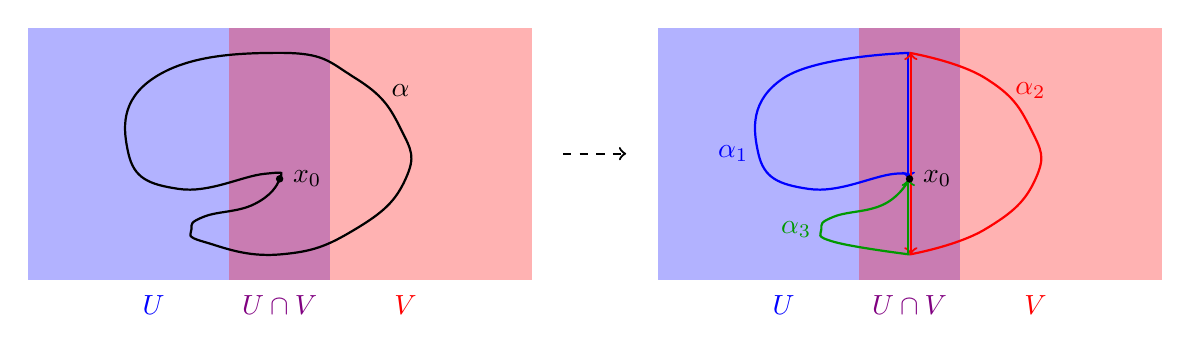
\begin{tikzpicture}[scale=0.8]
                \shorthandoff{>}

                \begin{scope}[shift={(-5,0)}, scale=0.8]
                    % Espacios
                    \path[fill=blue, opacity= 0.3] (1,0) rectangle (-5,5);
                    \node[blue] at (-2.5, -0.5) {$U$};
                    \path[fill=red, opacity= 0.3] (-1,0) rectangle (5,5);
                    \node[red] at (2.5, -0.5) {$V$};
                    \node[red!50!blue] at (0,-0.5) {$U \cap V$};

                    % Punto x_0
                    \node[draw, circle, fill=black, inner sep=0.8pt, label=right:{$x_0$}] at (0,2) {};

                    % Leyenda 
                    \node at (2.4,3.75) {$\alpha$};

                    % Arcos
                    \draw[black, thick] plot[smooth cycle, tension=0.8] coordinates {
                        (0,2) (-0.3,2.1) (-2,1.8) (-3,2.5) (-2.5, 4) (0,4.5) (1.5,4) (2.4,3) (2.5,2) (1.5,1) (0,0.5) (-1.5,0.75) (-1.75,1) (-1.5, 1.25) (-0.5, 1.5)
                    };
                \end{scope}

                % Flecha
                \draw[dashed, thick, ->] (-0.5, 2) -- (0.5, 2);

                \begin{scope}[shift={(5,0)}, scale=0.8]
                    % Espacios
                    \path[fill=blue, opacity= 0.3] (1,0) rectangle (-5,5);
                    \node[blue] at (-2.5, -0.5) {$U$};
                    \path[fill=red, opacity= 0.3] (-1,0) rectangle (5,5);
                    \node[red] at (2.5, -0.5) {$V$};
                    \node[red!50!blue] at (0,-0.5) {$U \cap V$};

                    % Arcos
                    \draw[blue, thick] plot[smooth, tension=0.8] coordinates {
                        (0,2) (-0.3,2.1) (-2,1.8) (-3,2.5) (-2.5, 4) (0,4.5)
                    };
                    \draw[red, thick] plot[smooth, tension=0.8] coordinates {
                        (0,4.5) (1.5,4) (2.4,3) (2.5,2) (1.5,1) (0,0.5)
                    };
                    \draw[green!60!black, thick] plot[smooth, tension=0.8] coordinates {
                        (0,0.5) (-1.5,0.75) (-1.75,1) (-1.5, 1.25) (-0.5, 1.5) (0,2)
                    };

                    % Leyenda 
                    \node[blue] at (-3.5, 2.5) {$\alpha_1$};
                    \node[red] at (2.4,3.75) {$\alpha_2$};
                    \node[green!60!black] at (-2.25,1) {$\alpha_3$};


                    % Cierres splines
                    \draw[blue, ->, thick] (-0.025,4.5) -- (-0.025,2);
                    \draw[red, <-, thick] (0.025,4.5) -- (0.025,2);
                    \draw[red, <-, thick] (0.025,0.5) -- (0.025,2);
                    \draw[green!60!black, ->, thick] (-0.025,0.5) -- (-0.025,2);

                    % Punto x_0
                    \node[draw, circle, fill=black, inner sep=0.8pt, label=right:{$x_0$}] at (0,2) {};
                \end{scope}

            \end{tikzpicture}
        \end{figure}

        Comenzamos con el lazo $\alpha:[0,1]\to X$. Consideramos $\alpha^{-1}(U)$ y $\alpha^{-1}(V)$ que son abiertos en $[0,1]$. Por el lema del número de Lebesgue tenemos que existen
        \begin{gather*}
            0=t_0 < t_1 < \dots < t_m = 1 \text{ partición del }[0,1]
        \end{gather*}
        
        tal que $\alpha([t_i, t_{i+1}])$ contenido en $U$ o bien en $V$ para $i\in\{0,\dots,m-1\}$. Si $\alpha(t_i)\notin U\cap V$ podemos quitar al $t_i$ de la partición ya que $\alpha([t_{i-1}, t_i]\cup [t_i, t_{i+1}])$ estaría contenido en $U$ o bien todo en $V$. Así suponemos todos los $\alpha(t_i)\in U\cap V$. Como $U\cap V$ es arcoconexo existe un arco $\beta_i$ uniendo $x_0$ con $\alpha(t_i)$ para cada $i\in \{1,\dots,m-1\}$. Tenemos por tanto
        \begin{gather*}
            [\alpha] = [\alpha_1\ast\alpha_2\ast\dots\ast\alpha_m]
        \end{gather*}
        donde $\alpha_i$ es una parametrización en $[0,1]$ de $\alpha|_{[t_{i-1}, t_i]}$. Tenemos que
        \begin{align*}
            [\alpha] &= [\alpha_1] \ast [\tilde{\beta}_1] \ast [\beta_1] \ast [\alpha_2]\ast[\tilde{\beta}_2] \ast \dots \ast [\beta_{m-1}] \ast [\alpha_m] =\\
            &= [\alpha_1 \ast \beta_1] \ast [\beta_1\ast \alpha_2 \ast \tilde{\beta_2}] \ast \dots \ast [\beta_{m-1}\ast \alpha_m]
        \end{align*}
        Donde $[\alpha_1\ast \tilde{\beta}_1]$, cada $[\beta_i \ast \alpha_{i+1} \ast \tilde{\beta}_{i+1}]$ y $[\beta_{m-1}\ast \alpha_m]$ son lazos basados en $x_0$ completamente contenidos en $U$ o bien en $V$.
    \end{proof}
\end{lema}

\begin{teo}
    Sean $X$ un e.t y $U,V$ abiertos de $X$. Supongamos que
    \begin{enumerate}
        \item $X=U\cup V$
        \item $U\cap V$ es arcoconexo (no vacío)
        \item $U$ y $V$ son simplemente conexos
    \end{enumerate}
    Entonces $X$ es simplemente conexo.
    \begin{proof}
        Dado $\alpha$ lazo basado en $x_0\in U\cup V$ se tiene por el lema anterior que 
        \begin{gather*}
            [\alpha] = [\alpha_1]\ast [\alpha_2] \ast \dots \ast [\alpha_k]
        \end{gather*}
        donde cada $\alpha_i$ es un lazo completamente contenido en $U$ o bien en $V$. Como $U,V$ son simplemente conexos tenemos
        \begin{gather*}
            [\alpha] = [\veps_{x_0}]\ast[\veps_{x_0}]\ast \dots \ast [\veps_{x_0}] = [\veps_{x_0}]
        \end{gather*}
    \end{proof}
\end{teo}

\begin{coro}
    Las esferas $\bb{S}^n$ para $n\geq 2$ con simplemente conexas.En particular su grupo fundamental es el trivial.

    \begin{proof}
        Definimos los siguientes conjuntos
        \begin{gather*}
            U=\bb{S}^n \setminus \{(0,\dots,1)\} \hspace{2cm} 
            V = \bb{S}^n \setminus \{(1,\dots,0)\}
        \end{gather*}
        $U$ y $V$ son homeomorfos a $\bb{R}^n$ por lo que son simplemente conexos, $\bb{S}^n=U\cup V$ y además, como $U\cap V$ es homeomorfo a $\bb{R}^n \setminus \{(0,\dots,0)\}$ que es arcoconexo (ya que $n\geq 2$), tenemos que $U\cap V$ es arcoconexo.
    \end{proof}
\end{coro}

\begin{coro}
    El grupo fundamental de $\bb{R}P^n$ $\bb{R}\cc{P}^n$ es isomorfo a $\bb{Z}^2$ para $n\geq 2$.

    \begin{proof}\
        \begin{figure}[H]
            \centering
            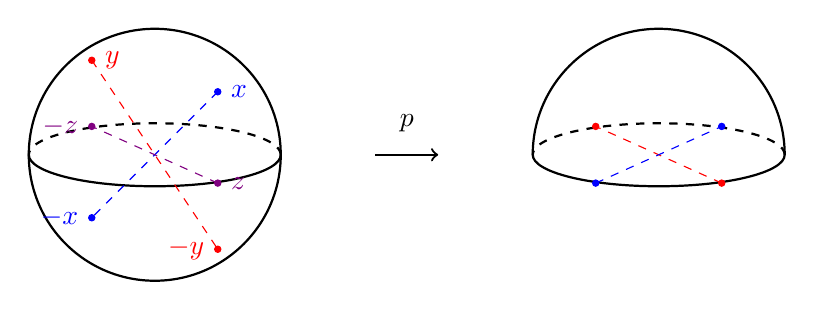
\begin{tikzpicture}[scale=0.8]
                \shorthandoff{>}

                \begin{scope}[shift={(-4,0)}]
                    % Circunferencia
                    \draw[thick] (0,0) circle [radius=2];
                    \draw[thick, dashed] (2,0) arc (0:180:2 and 0.5);
                    \draw[thick] (2,0) arc (0:-180:2 and 0.5);

                    % Puntos
                    \node[draw, circle, fill=blue, blue, inner sep=0.8pt, label={[blue]right:{$x$}}] at (1,1) {};
                    \node[draw, circle, fill=blue, blue, inner sep=0.8pt, label={[blue]left:{$-x$}}] at (-1,-1) {};
                    \draw[dashed, blue] (1,1) -- (-1,-1);

                    \node[draw, circle, fill=red, red, inner sep=0.8pt, label={[red]right:{$y$}}] at (-1,1.5) {};
                    \node[draw, circle, fill=red, red, inner sep=0.8pt, label={[red]left:{$-y$}}] at (1,-1.5) {};
                    \draw[dashed, red] (-1,1.5) -- (1,-1.5);

                    \node[draw, circle, fill=violet, violet, inner sep=0.8pt, label={[violet]right:{$z$}}] at (1,-0.45) {};
                    \node[draw, circle, fill=violet, violet, inner sep=0.8pt, label={[violet]left:{$-z$}}] at (-1,0.45) {};
                    \draw[dashed, violet] (1,-0.45) -- (-1,0.45);

                \end{scope}

                % Función p
                \draw[->, thick] (-0.5,0) -- (0.5,0);
                \node at (0,0.5) {$p$};

                \begin{scope}[shift={(4,0)}]
                    % Circunferencia
                    \draw[thick] (2,0) arc (0:180:2 and 2);
                    \draw[thick, dashed] (2,0) arc (0:180:2 and 0.5);
                    \draw[thick] (2,0) arc (0:-180:2 and 0.5);

                    % Puntos
                    \node[draw, circle, fill=red, red, inner sep=0.8pt] at (1,-0.45) {};
                    \node[draw, circle, fill=red, red, inner sep=0.8pt] at (-1,0.45) {};
                    \draw[dashed, red] (1,-0.45) -- (-1,0.45);


                    \node[draw, circle, fill=blue, blue, inner sep=0.8pt] at (-1,-0.45) {};
                    \node[draw, circle, fill=blue, blue, inner sep=0.8pt] at (1,0.45) {};
                    \draw[dashed, blue] (-1,-0.45) -- (1,0.45);

                \end{scope}

            \end{tikzpicture}
        \end{figure}

        Veamos que la aplicación
        \begin{align*}
            p: \bb{S}^n & \to \bb{R}P^n\\
            x & \mapsto [x]
        \end{align*}
        es recubridora. Es claro que $p$ es continua y sobreyectiva. Por otro lado, dado cualquier punto $x_0\in \bb{S}^n$ tenemos que el abierto
        \begin{gather*}
            U_{x_0} = \{x\in \bb{S}^n : \langle x, x_0 \rangle \neq 0\}
        \end{gather*}
        es saturado, es decir, que $p^{-1}(p(U_{x_0})) = U_{x_0}$) y además podemos escribir
        \begin{gather*}
            U_{x_0} = \{x\in \bb{S}^n : \langle x, x_0 \rangle > 0\} \cup \{x\in \bb{S}^n : \langle x, x_0 \rangle < 0\} = U_{x_0}^+ \cup U_{x_0}^-
        \end{gather*}
        Es fácil probar que $p|_{U_{x_0}^+}$ y $p|_{U_{x_0}^-}$ son homeomorfismos. Entonces la correspondencia del levantamiento
        \begin{gather*}
            \varphi: \pi_1(\bb{R}P^n, [a_0]) \to p^{-1}([a_0]) = \{a_0,-a_0\}
        \end{gather*}
        es biyectiva (ya que $\bb{S}^1$ es simplemente conexo). Entonces $\pi_1(\bb{R}P^n, [a_0])$ solo tiene dos elementos, luego $\pi_1(\bb{R}P^n, [a_0]) \cong \bb{Z}^2$.
    \end{proof}
\end{coro}

\begin{ejemplo}\
    \begin{enumerate}
        \item Calculamos el grupo fundamental de dos esferas $S_1, S_2$ de $\bb{R}^3$ que se cortan en un único punto.
        
        \begin{figure}[H]
            \centering
            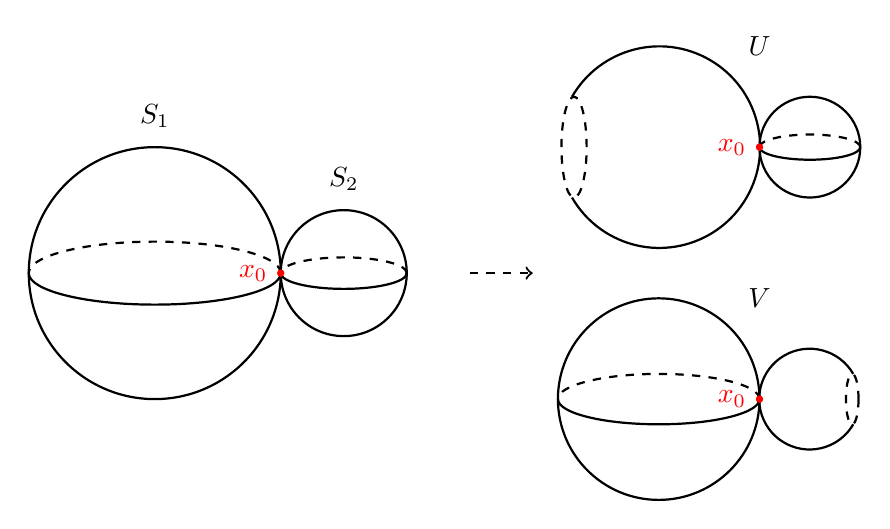
\begin{tikzpicture}[scale=0.8]
                \shorthandoff{>}

                \begin{scope}[shift={(-5,0)}]
                    % Circunferencia 1
                    \draw[thick] (0,0) circle [radius=2];
                    \draw[thick, dashed] (2,0) arc (0:180:2 and 0.5);
                    \draw[thick] (2,0) arc (0:-180:2 and 0.5);

                    % Circunferencia 2
                    \draw[thick] (3,0) circle [radius=1];
                    \draw[thick, dashed] (4,0) arc (0:180:1 and 0.25);
                    \draw[thick] (4,0) arc (0:-180:1 and 0.25);

                    % Leyenda
                    \node at (0,2.5) {$S_1$};
                    \node at (3,1.5) {$S_2$};

                    % Intersección
                    \node[draw, circle, fill=red, red, inner sep=0.8pt, label={[red]left:{$x_0$}}] at (2,0) {};
                \end{scope}

                \draw[->, thick, dashed] (0,0) -- (1,0);

                \begin{scope}[shift={(3,2)}, scale=0.8]
                    % Circunferencia 1
                    \draw[thick, dashed] (-1.68,0) ellipse (0.25 and 1);
                    \draw[thick] (-1.72,1) arc (150:-150:2 and 2);

                    % Circunferencia 2
                    \draw[thick] (3,0) circle [radius=1];
                    \draw[thick, dashed] (4,0) arc (0:180:1 and 0.25);
                    \draw[thick] (4,0) arc (0:-180:1 and 0.25);

                    % Leyenda
                    \node at (2,2) {$U$};

                    % Intersección
                    \node[draw, circle, fill=red, red, inner sep=0.8pt, label={[red]left:{$x_0$}}] at (2,0) {};
                \end{scope}

                \begin{scope}[shift={(3,-2)}, scale=0.8]
                    % Circunferencia 1
                    \draw[thick] (0,0) circle [radius=2];
                    \draw[thick, dashed] (2,0) arc (0:180:2 and 0.5);
                    \draw[thick] (2,0) arc (0:-180:2 and 0.5);

                    % Circunferencia 2                    
                    \draw[thick, dashed] (3.84,0) ellipse (0.125 and 0.5);
                    \draw[thick] (3.86,0.5) arc (30:330:1 and 1);

                    % Leyenda
                    \node at (2,2) {$V$};

                    % Intersección
                    \node[draw, circle, fill=red, red, inner sep=0.8pt, label={[red]left:{$x_0$}}] at (2,0) {};
                \end{scope}

            \end{tikzpicture}
        \end{figure}
        
        Sea $\{x_0\} = S_1\cap S_2$ y tomamos $U=X\setminus\{y_1\}$ con $y_1\in S_1\setminus\{x_0\}$ y $V=X\setminus\{y_2\}$ con $y_2\in S_2\setminus\{x_0\}$. Es claro que $X=U \cap V$ y $U,V$ son abiertos. $U\cap V$ es arcoconexo por ser unión de dos arcoconexos $(S_1\setminus\{y_1\})\cup (S_2\setminus\{y_2\})$ ya que 
        \begin{gather*}
            S_1\setminus\{y_1\} \text{ homeomorfo a } \bb{R}^2 \Rightarrow S_1\setminus\{y_1\} \text{ es arcoconexo}\\
            S_2\setminus\{y_2\} \text{ homeomorfo a } \bb{R}^2 \Rightarrow S_2\setminus\{y_2\} \text{ es arcoconexo}
        \end{gather*}
        y que tienen un punto común $x_0$. Veamos ahora que $U$ tiene a $S_2$ por retracto de deformación. Si esto es cierto, entonces 
        \begin{gather*}
            \pi(U)\overset{\text{isom.}}{\cong}\pi_1(S_2)\cong \{0\}
        \end{gather*}
        Sabemos que $S_1\setminus\{y_1\}$ es homeomorfo a $\bb{R}^2$ y podemos suponer que la imagen mediante ese homeomorfosmo de $x_0$ es el origen $(0,0)$. Entonces la composición de este homeomorfismo y la homotopía 
        \begin{gather*}
            H(x,t) = (1-t)x \ \ \ x\in \bb{R}^2
        \end{gather*}
        nos da una homotopía $\hat{H}:(S_1\setminus \{y_1\}) \times [0,1] \to S_1\setminus \{y_1\}$ tal que $\hat{H}(x_0,t)=x_0$. Entonces
        \begin{align*}
            \tilde{H}:U \times [0,1] &\to U\\
            (x,t) & \mapsto \left\{
                \begin{array}{l c c}
                    \hat{H}(x,t) & \text{ si } & x\in S_1\setminus \{y_1\}\\
                    x & \text{ si } & x\in S_2
                \end{array}
            \right.
        \end{align*}
        es una homotopía desde la identidad hasta la que deja fijos a todos los puntos de $S_1$, luego $S_2$ es un retracto de deformación de $U$.

        \item Si llamamos $S(x,r)$ a la esfera centrada en $x\in \bb{R}^3$ de radio $r>0$ y consideramos
        \begin{gather*}
            X = \bigcup\limits_{k\in \bb{Z}} S\left((k,0,0), \frac{1}{2}\right)
        \end{gather*}
        veamos que su grupo fundamental es el trivial.

        \begin{figure}[H]
            \centering
            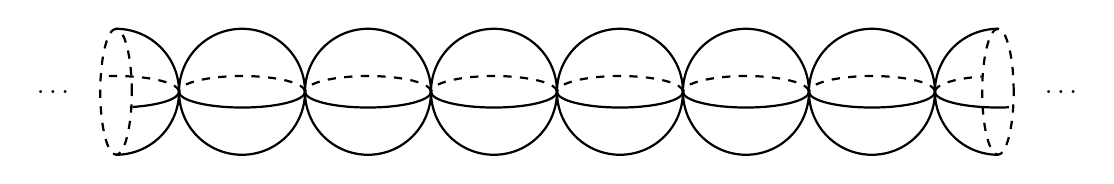
\begin{tikzpicture}[scale=0.8]
                \shorthandoff{>}

                \node at (-3,0) {$\dots$};

                \begin{scope}[shift={(-2,0)}]
                        % Circunferencia
                        \draw[thick] (0,1) arc (90:-90:1 and 1);
                        \draw[dashed, thick] (0,0) ellipse (0.25 and 1);
                        \draw[thick, dashed] (1,0) arc (0:100:1 and 0.25);
                        \draw[thick] (1,0) arc (0:-75:1 and 0.25);
                \end{scope}

                % Cadena de circunferencias
                \foreach \x in {0,2,...,10} {
                    \begin{scope}[shift={(\x,0)}]
                        % Circunferencia
                        \draw[thick] (0,0) circle [radius=1];
                        \draw[thick, dashed] (1,0) arc (0:180:1 and 0.25);
                        \draw[thick] (1,0) arc (0:-180:1 and 0.25);
                    \end{scope}
                }

                \begin{scope}[shift={(12,0)}]
                        % Circunferencia
                        \draw[thick] (0,1) arc (90:270:1 and 1);
                        \draw[dashed, thick] (0,0) ellipse (0.25 and 1);
                        \draw[thick, dashed] (-1,0) arc (180:105:1 and 0.25);
                        \draw[thick] (-1,0) arc (180:280:1 and 0.25);
                \end{scope}

                \node at (13,0) {$\dots$};

            \end{tikzpicture}
        \end{figure}

        Para ello, con una simple inducción se puede demostrar que esto es cierto para una cantidad finita de esferas usando el ejemplo anterior. En este caso tenemos una cantidad infinita de esferas pero como un lazo es un compacto en $\bb{R}^3$, tiene que caer en una unión finita de esferas (unidas dos a dos por un único punto) por lo que se podrá reducir al trivial.


        \item Vamos a definir el siguiente conjunto
        \begin{gather*}
            X = \bb{S}^2 \cup \{(x,y,0) : x^2 + y^2 \leq 1\}
        \end{gather*}
        y veamos cual es su grupo fundamental.

        \begin{figure}[H]
            \centering
            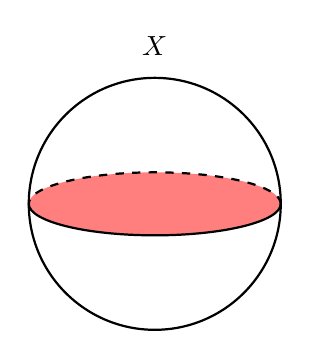
\begin{tikzpicture}[scale=0.8]
                \shorthandoff{>}

                \fill[red, opacity=0.5] (0,0) ellipse (2 and 0.5);

                \draw[thick] (0,0) circle [radius=2];
                \draw[thick, dashed] (2,0) arc (0:180:2 and 0.5);
                \draw[thick] (2,0) arc (0:-180:2 and 0.5);

                \node at (0,2.5) {$X$};

            \end{tikzpicture}
        \end{figure}

        Para ello tomamos $U=X\setminus \{(0,0,1)\}$ que es retracto de deformación de $U_1$ donde
        \begin{gather*}
            U_1 = \{(x_1,x_2,x_3)\in \bb{S}^2 : x_3 \leq 0\}\cup \{(x,y,0) : x^2 + y^2 \leq 1\}
        \end{gather*}
        y además $U_1$ es homeomorfo a $\bb{S}^2$ por lo que $\pi_1(U)$ es el trivial. 
        
        \begin{figure}[H]
            \centering
            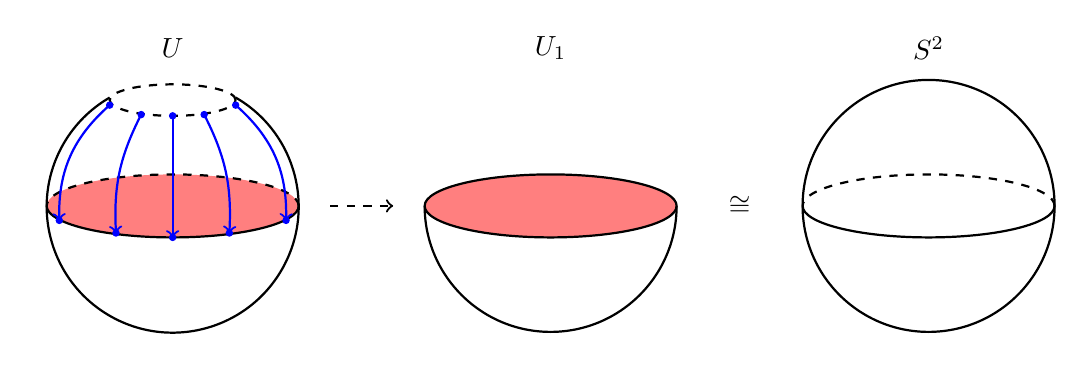
\begin{tikzpicture}[scale=0.8]
                \shorthandoff{>}

                \begin{scope}[shift={(-2,0)}]
                    \node at (0,2.5) {$U$};

                    % Color radio medio
                    \fill[red, opacity=0.5] (0,0) ellipse (2 and 0.5);

                    % Radio medio
                    \draw[thick, dashed] (2,0) arc (0:180:2 and 0.5);
                    \draw[thick] (2,0) arc (0:-180:2 and 0.5);

                    % Agujero superior
                    \draw[thick, dashed] (0,1.68) ellipse (1 and 0.25);
                    \draw[thick] (1, 1.72) arc (60:-240:2 and 2);

                    % Puntos superiores
                    \node[draw, circle, fill=blue, blue, inner sep=0.8pt] at (-1,1.6) {};
                    \node[draw, circle, fill=blue, blue, inner sep=0.8pt] at (-0.5,1.45) {};
                    \node[draw, circle, fill=blue, blue, inner sep=0.8pt] at (0,1.43) {};
                    \node[draw, circle, fill=blue, blue, inner sep=0.8pt] at (0.5,1.45) {};
                    \node[draw, circle, fill=blue, blue, inner sep=0.8pt] at (1,1.6) {};

                    % Puntos inferiores
                    \node[draw, circle, fill=blue, blue, inner sep=0.8pt] at (-1.8,-0.23) {};
                    \node[draw, circle, fill=blue, blue, inner sep=0.8pt] at (-0.9,-0.43) {};
                    \node[draw, circle, fill=blue, blue, inner sep=0.8pt] at (0,-0.5) {};
                    \node[draw, circle, fill=blue, blue, inner sep=0.8pt] at (0.9,-0.43) {};
                    \node[draw, circle, fill=blue, blue, inner sep=0.8pt] at (1.8,-0.23) {};
                    
                    % Arcos con flecha
                    \draw[->, bend right=25, blue, thick] (-1,1.6) to (-1.8,-0.23);
                    \draw[->, bend right=15, blue, thick] (-0.5,1.45) to (-0.9,-0.43);
                    \draw[->, blue, thick] (0,1.43) to (0,-0.5);
                    \draw[->, bend left=15, blue, thick] (0.5,1.45) to (0.9,-0.43);
                    \draw[->, bend left=25, blue, thick] (1,1.6) to (1.8,-0.23);
                \end{scope}

                \draw[->, dashed, thick] (0.5,0) -- (1.5,0);

                \begin{scope}[shift={(4,0)}]
                    \node at (0,2.5) {$U_1$};

                    % Radio medio
                    \fill[red, opacity=0.5] (0,0) ellipse (2 and 0.5);
                    \draw[thick] (0,0) ellipse (2 and 0.5);

                    % Circunferencia
                    \draw[thick] (2,0) arc (0:-180:2 and 2);
                \end{scope}

                \node at (7,0) {$\cong$};

                \begin{scope}[shift={(10,0)}]
                    \node at (0,2.5) {$\bb{S}^2$};

                    %Circunferencia
                    \draw[thick] (0,0) circle [radius=2];

                    % Radio medio
                    \draw[thick, dashed] (2,0) arc (0:180:2 and 0.5);
                    \draw[thick] (2,0) arc (0:-180:2 and 0.5);
                \end{scope}

            \end{tikzpicture}
        \end{figure}
        
        De forma análoga si consideramos $V=X\setminus \{(0,0,-1)\}$ se tiene que $\pi_1(V)$ es trivial. Claramente se tiene que $U\cap V$ es arcoconexo\footnote{en un examen habrá que demostrarlo de forma más rigurosa} y por el teorema anterior se tiene que $X$ es simplemente conexo, luego su grupo fundamental es el trivial.
    \end{enumerate}
\end{ejemplo}

\begin{lema}
    Sea $f:\bb{S}^1 \to \bb{S}^1$ una aplicación continua que conserva antípodas, es decir, $f(-x)=-x$ para todo $x\in \bb{S}^1$. Si consideramos el lazo
    \begin{gather*}
        \alpha(s) = (\cos(2\pi s), \sen(2\pi s))
    \end{gather*}
    entonces se tiene que el grado del lazo $f\circ \alpha$ es impar.
    \begin{proof}
        La curva $\alpha$ la podemos ver como $\alpha = \alpha_1 \ast \alpha_2$ con
        \begin{gather*}
            \alpha_1(s) = \alpha\left(\frac{s}{2}\right) \ \ \ s\in[0,1]\\
            \alpha_2(s) = \alpha\left(\frac{s+1}{2}\right) \ \ \ s\in[0,1]
        \end{gather*}
        Como $(f \circ \alpha_1)$ es un arco que comienza en $(1,0)$ y acaba en $(-1,0)$, entonces su levantamiento por $p$ lo podemos elegir para que comience en $0$ (ya que $p(0)=(1,0)$) y un punto final $\tilde{(f \circ \alpha_1)}(1)$ que ha de cumplir que $p(\tilde{(f\circ \alpha_1)}(1))=(-1,0)$. Es decir,
        \begin{gather*}
            \cos(2\pi (\tilde{(f\circ \alpha_1)}(1))) = -1\\
            \sen(2\pi (\tilde{(f\circ \alpha_1)}(1))) = 0
        \end{gather*}
        y tenemos que $(\tilde{f\circ \alpha}(1)) = k + \frac{1}{2}$ para un cierto $k\in \bb{Z}$. Veamos que $\tilde{f\circ \alpha}$ es la siguiente curva
        \begin{gather*}
            \tilde{f\circ \alpha} = \tilde{f\circ \alpha_1} \ast \gamma
        \end{gather*}
        donde $\gamma(s) = k + \frac{1}{2} + \tilde{f\circ \alpha_1}$.\\

        Tenemos que comprobar que $\tilde{f\circ \alpha_1} \ast \gamma$ está bien definida, lo cual es claro porque
        \begin{gather*}
            (\tilde{f\circ \alpha_1})(1) = k + \frac{1}{2} = k + \frac{1}{2} + (\tilde{f\circ \alpha_1})(0) = \gamma(0)
        \end{gather*}
        y que $p(\tilde{f\circ \alpha_1} \ast \gamma) = f \circ \alpha$. Tenemos que 
        \begin{gather*}
            p((\tilde{f\circ \alpha_1}) \ast \gamma) = p(\tilde{f\circ \alpha_1}) \ast p(\gamma) = (f\circ \alpha_1) \ast p(\gamma)
        \end{gather*}
        y si desarrollamos tenemos
        \begin{align*}
            p(\gamma) &= p\left(k+\frac{1}{2} + (\tilde{f\circ \alpha_1})(s) \right) =\\
            &= \left(\cos\left(2\pi \left(k + \frac{1}{2} + (\tilde{f\circ \alpha_1})(s)\right)\right), \sen\left(2\pi \left(k + \frac{1}{2} + (\tilde{f\circ \alpha_1})(s)\right)\right)\right) = \\
            &= (\cos (\pi + 2 \pi (\tilde{f\circ \alpha_1})(s)), \sen (\pi + 2 \pi (\tilde{f\circ \alpha_1})(s))) = \\
            &=-(\cos (2\pi(\tilde{f\circ \alpha_1})(s)), \sen (2 \pi (\tilde{f\circ \alpha_1})(s))) = \\
            &= -p((\tilde{f\circ \alpha_1})(s)) = -(f\circ \alpha_1)(s) \overset{hip.}{=} f(-\alpha_1(s)) =\\
            &= f(\alpha_2(s))
        \end{align*}
        y llegamos a que $p(\tilde{f\circ \alpha_1} \ast \gamma) = (f\circ \alpha_1) \ast (f\circ \alpha_2) = f \circ \alpha$. Por tanto finalmente tenemos
        \begin{gather*}
            \deg(f\circ \alpha) = (\tilde{f\circ \alpha})(1) = \gamma(1) = k + \frac{1}{2} + (\tilde{f\circ \alpha_1})(1)=\\
            =\left(k + \frac{1}{2}\right) + \left(k+\frac{1}{2}\right) = 2k + 1 \text{ impar}
        \end{gather*}
    \end{proof}
\end{lema}

\begin{lema}
    No existe una aplicación continua $f:\bb{S}^2\to \bb{S}^1$ que conserve antípodas, es decir, tal que $f(-x)=-f(x)$ para todo $x\in \bb{S}^2$.

    \begin{proof}\

        \begin{figure}[H]
            \centering
            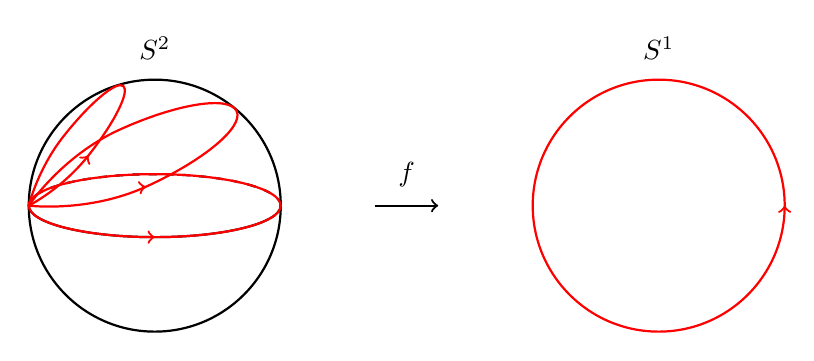
\begin{tikzpicture}[scale=0.8]
                \shorthandoff{>}

                \begin{scope}[shift={(-4,0)}]
                    \node at (0,2.5) {$\bb{S}^2$};

                    % Circunferencia
                    \draw[thick] (0,0) circle [radius=2];

                    % Radio medio
                    \draw[thick, dashed] (2,0) arc (0:180:2 and 0.5);
                    \draw[thick] (2,0) arc (0:-180:2 and 0.5);

                    % Arcos
                    \draw[thick, red] (0,0) ellipse (2 and 0.5);
                    \draw[->, red, thick] (0,-0.5) ++(-0.01, 0) -- ++(0.01,0);

                    \draw[red, thick] plot[smooth, tension=1] coordinates {
                        (-2,0) (-0.14,0.3) (1.3,1.5) (-0.56,1.205) (-2,0)
                    };
                    \draw[->, red, thick] (-0.14,0.3) ++(-0.065, -0.01) -- ++(+0.065,0.01);

                    \draw[red, thick] plot[smooth, tension=1] coordinates {
                        (-2,0) (-1.0537,0.795) (-0.5,1.9) (-1.446,1.104) (-2,0)
                    };
                    \draw[->, red, thick] (-1.0537,0.795) ++(-0.007, -0.01) -- ++(+0.007,0.01);
                    
                \end{scope}

                \node at (0,0.5) {$f$};
                \draw[->, thick] (-0.5,0) -- (0.5,0);

                \begin{scope}[shift={(4,0)}]
                    \node at (0,2.5) {$\bb{S}^1$};

                    % Circunferencia
                    \draw[thick, red] (0,0) circle [radius=2];

                    \draw[->, red, thick] (2,0) ++(0, -0.01) -- ++(0,0.01);
                \end{scope}
            \end{tikzpicture}
        \end{figure}

        Supongamos que existiese $f:\bb{S}^2 \to \bb{S}^1$ continua con $f(-x) = -f(x)$\ \ $\forall x \in \bb{S}^2$. Entonces consideramos la aplicación 
        \begin{align*}
            j: \bb{S}^1 & \to \bb{S}^2\\
            (x,y) & \mapsto (x,y)
        \end{align*}
        que es continua. 
        
        \begin{figure}[H]
            \centering
            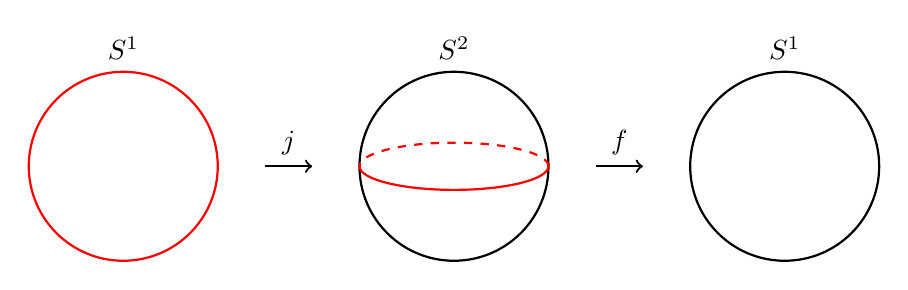
\begin{tikzpicture}[scale=0.6]
                \shorthandoff{>}

                \begin{scope}[shift={(-7,0)}]
                    \node at (0,2.5) {$\bb{S}^1$};

                    % Circunferencia
                    \draw[thick, red] (0,0) circle [radius=2];
                    
                \end{scope}

                \node at (-3.5,0.5) {$j$};
                \draw[->, thick] (-4,0) -- (-3,0);

                \begin{scope}[shift={(0,0)}]
                    \node at (0,2.5) {$\bb{S}^2$};

                    % Circunferencia
                    \draw[thick] (0,0) circle [radius=2];

                    % Radio medio
                    \draw[thick, red, dashed] (2,0) arc (0:180:2 and 0.5);
                    \draw[thick, red] (2,0) arc (0:-180:2 and 0.5);
                \end{scope}

                \node at (3.5,0.5) {$f$};
                \draw[->, thick] (3,0) -- (4,0);

                \begin{scope}[shift={(7,0)}]
                    \node at (0,2.5) {$\bb{S}^1$};

                    % Circunferencia
                    \draw[thick] (0,0) circle [radius=2];
                \end{scope}
            \end{tikzpicture}
        \end{figure}
        
        Tenemos además que $f\circ j : \bb{S}^1 \to \bb{S}^1$ conserva antípodas (salvo rotación de $\bb{S}^1$ podemos suponer que $(f\circ j)(1,0)=(1,0)$). Por el lema anterior tenemos que existe un lazo $\alpha$ tal que $\deg((f\circ j)(\alpha))$ es impar. En particular se tiene que 
        \begin{align*}
            (f\circ j)_*([\alpha]) &\neq [\veps_{(1,0)}]\\
            (f\circ j)_*([\alpha]) &= (f_* \circ j_*)([\alpha]) = [\veps_{(1,0)}]
        \end{align*}
        lo que contradice la existencia de $f$ continua.
    \end{proof}
\end{lema}

\begin{teo}[Teorema de Borsuk-Ulam]
    Sea $f:\bb{S}^2 \to \bb{R}^2$ una aplicación continua. Entonces existe $x_0\in \bb{S}^2$ tal que $f(x_0)=f(-x_0)$.

    \begin{proof}
        Si no existiese $x\in \bb{S}^2$ tal que $f(x)=f(-x)$, entonces podríamos considerar 
        \begin{gather*}
            g(x) = \frac{f(x)-f(-x)}{|f(x)-f(-x)|} \text{ continua de $\bb{S}^2$ en $\bb{S}^1$}
        \end{gather*}
        y se tendría que $g(-x)=-g(x)$, lo que contradice el lema anterior.
    \end{proof}
\end{teo}

\begin{observacion}
    Del teorema de Borsuk-Ulam se deduce que no existen aplicaciones continuas e inyectivas de $\bb{S}^2$ en $\bb{R}^2$. Se deduce que $\bb{S}^2$ no es homeomorfo a ningún subconjunto de $\bb{R}^2$.
\end{observacion}

\begin{teo}[de las tortitas]
    Sean $A_1$ y $A_2$ dos compactos de $\bb{R}^2$, entonces existe una única que divide a ambos a la vez dejando la mitad del área de cada uno a cada lado de la recta.

    \begin{figure}[H]
        \centering
        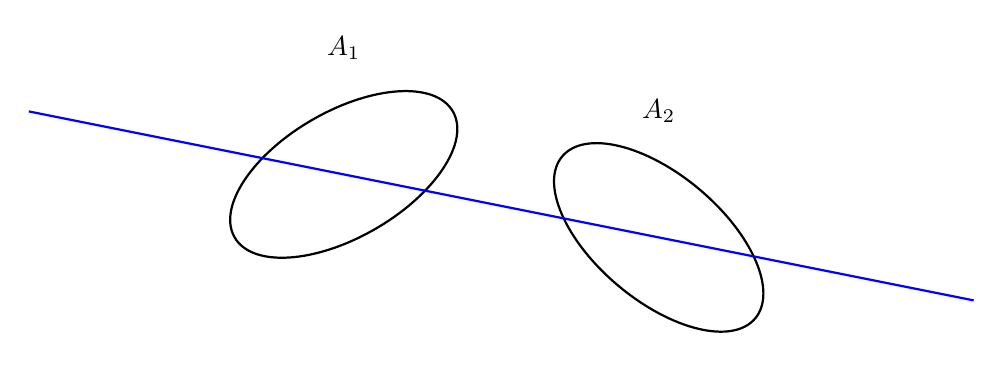
\begin{tikzpicture}[scale=0.8]
            \shorthandoff{>}

            \node at (-2,2) {$A_1$};
            \node at (3,1) {$A_2$};

            \draw[thick, rotate around={30:(-2,0)}] (-2,0) ellipse (2 and 1);
            \draw[thick, rotate around={-40:(3,-1)}] (3,-1) ellipse (2 and 1);

            \draw[thick, blue] (-7,1) -- (8,-2);
        \end{tikzpicture}
    \end{figure}

    \begin{proof}
        Identificamos $\bb{R}^2$ dentro de $\bb{R}^3$ como $\bb{R}^2 \times \{1\}$. Para cada $x\in \bb{S}^2$ consideramos
        \begin{gather*}
            P_x^+ = \{v\in \bb{R}^3 : \langle v,x \rangle > 0\}\\
            P_x^- = \{v\in \bb{R}^3 : \langle v,x \rangle < 0\}\\
            L_x = \{v\in \bb{R}^3 : \langle v,x \rangle = 0\} \cap (\bb{R}^2\times\{1\})
        \end{gather*}

        \begin{figure}[H]
            \centering
            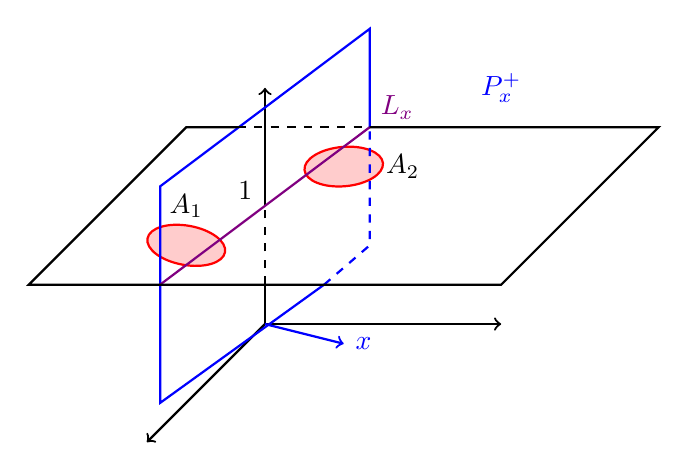
\begin{tikzpicture}
                \shorthandoff{>}

                % Ejes
                \draw[thick, <-] (-1.5,-1.5) -- (0,0);
                \draw[thick] (0,0) -- (0,0.5);
                \draw[thick, dashed] (0,0.5) -- (0,1.5);
                \draw[thick, ->] (0,1.5) -- (0,3);
                \draw[thick, ->] (0,0) -- (3,0);

                \node at (-0.25,1.7) {$1$};

                % Vector x
                \draw[thick, blue, ->] (0,0) -- (1, -0.25);
                \node[blue] at (1.25, -0.25) {$x$};

                % Compactos
                \draw[thick, red, fill=red!20, rotate around={-10:(-1,1)}] (-1,1) ellipse (0.5 and 0.25);
                \node at (-1,1.5) {$A_1$};

                \draw[thick, red, fill=red!20, rotate around={5:(1,2)}] (1,2) ellipse (0.5 and 0.25);
                \node at (1.75,2) {$A_2$};

                % Plano perpendicular
                \draw[thick, blue] (1.33,2.5) -- (1.33,3.75) -- (-1.33,1.75) -- (-1.33,-1) -- (0.75,0.5);
                \draw[thick, blue, dashed] (0.75,0.5) -- (1.33,1) -- (1.33,2.5);
                \draw[thick, violet] (-1.333,0.5) -- (1.33,2.5);
                \node[violet] at (1.68,2.75) {$L_x$};
                \node[blue] at (3,3) {$P_x^+$};

                % Plano horizontal
                \draw[thick] (1.33,2.5) -- (5,2.5) -- (3,0.5) -- (-3,0.5) -- (-1,2.5) -- (-0.35,2.5);
                \draw[thick, dashed] (-0.35,2.5) -- (1.33,2.5);
                
            \end{tikzpicture}
        \end{figure}

        Observamos que si $x\neq \pm (0,0,1)$, entonces $L_x$ es una recta. En otro caso, si $x= \pm (0,0,1)$, entonces $L_x=\emptyset$. Observemos además que $P_x^+=P_{-x}^-$. Además, si $area(A_1)=area(A_2)=0$, entonces cualquier recta nos vale. Vamos a suponer entonces que $area(A_1)>0$ y definimos
        \begin{align*}
            f: \bb{S}^2 & \to \bb{R}^2\\
            x & \mapsto (area(A_1\cap P_x^+), area(A_2\cap P_x^+))
        \end{align*}
        Como $f$ es continua, entonces el teorema de Borsuk Ulam $\exists x_0\in \bb{S}^2$ tal que $f(x_0)=f(-x_0)$, es decir, tal que
        \begin{gather*}
            (area(A_1\cap P_{x_0}^+), area(A_2\cap P_{x_0}^+)) = (area(A_1\cap P_{x_0}^-), area(A_2\cap P_{x_0}^-))
        \end{gather*}
        por lo que llegamos a que 
        \begin{gather*}
            \left\{
                \begin{array}{l}
                    area(A_1\cap P_{x_0}^+) = area(A_1\cap P_{x_0}^-)\\
                    area(A_2\cap P_{x_0}^+) = area(A_2\cap P_{x_0}^-)
                \end{array}
            \right.
        \end{gather*}
        (recordemos que $x_0\neq (0,0,1)$).
    \end{proof}
\end{teo}

\begin{teo}[del bocadillo de jamón]
    Sean $A_1$, $A_2$, $A_3$ tres compactos en $\bb{R}^3$, entonces existe un plano que divide a la vez a cada uno de ellos en dos partes de igual volumen.

    \begin{figure}[H]
        \centering
        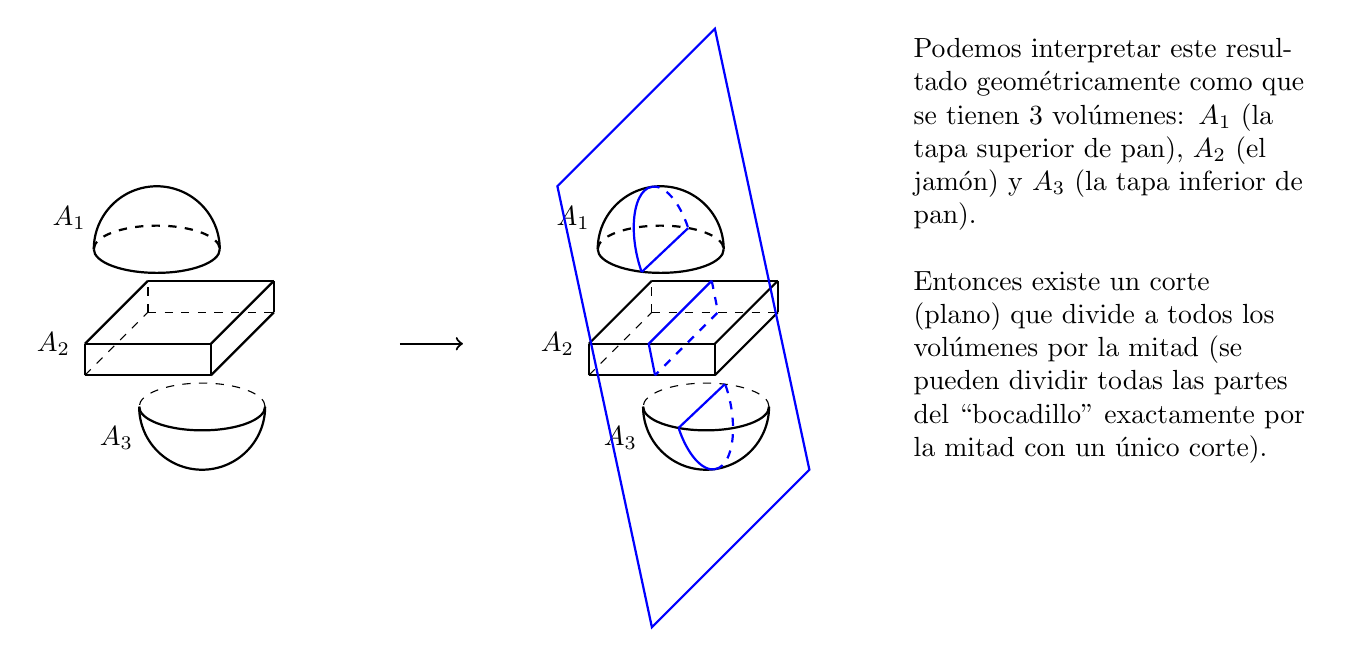
\begin{tikzpicture}[scale=0.4]
            \shorthandoff{>}

            \begin{scope}[shift={(-8,0)}]

                \node at (-3.5,4) {$A_1$};
                \node at (-4,0) {$A_2$};
                \node at (-2,-3) {$A_3$};

                % Tapa superior
                \begin{scope} [shift={(-0.72,3)}, rotate=180]
                    \draw[thick] (2,0) arc (0:180:2 and 0.75);
                    \draw[dashed, thick] (2,0) arc (0:-180:2 and 0.75);
                    \draw[thick] (2,0) arc (0:-180:2 and 2); 
                \end{scope}

                % Jamón
                \draw[dashed] (-1,1) -- (-1,2);
                \draw[dashed] (-1,1) -- (3,1);
                \draw[thick] (3,1) -- (3,2);
                \draw[thick] (-1,2) -- (3,2);
                \draw[thick] (-3,-1) -- (-3,0);
                \draw[thick] (-3,-1) -- (1,-1);
                \draw[thick] (1,-1) -- (1,0);
                \draw[thick] (-3,0) -- (1,0);
                \draw[dashed] (-3,-1) -- (-1,1);
                \draw[thick] (-3,0) -- (-1,2);
                \draw[thick] (1,-1) -- (3,1);
                \draw[thick] (1,0) -- (3,2);

                % Tapa inferior
                \begin{scope} [shift={(0.72,-2)}]
                    \draw[dashed] (2,0) arc (0:180:2 and 0.75);
                    \draw[thick] (2,0) arc (0:-180:2 and 0.75);
                    \draw[thick] (2,0) arc (0:-180:2 and 2); 
                \end{scope}

            \end{scope}

            \draw[thick, ->] (-1, 0) -- (1,0); 

            \begin{scope}[shift={(8,0)}]

                \node at (-3.5,4) {$A_1$};
                \node at (-4,0) {$A_2$};
                \node at (-2,-3) {$A_3$};

                % Tapa superior
                \begin{scope} [shift={(-0.72,3)}, rotate=180]
                    \draw[thick] (2,0) arc (0:180:2 and 0.75);
                    \draw[dashed, thick] (2,0) arc (0:-180:2 and 0.75);
                    \draw[thick] (2,0) arc (0:-180:2 and 2); 
                    \draw[thick, blue, dashed, rotate=12] (-0.12,-2) arc (-90:-166:0.9 and 2);
                    \draw[thick, blue, rotate=12] (-0.12,-2) arc (-90:17:0.9 and 2);  
                    \draw[thick, blue] (-0.87,-0.67) -- (0.6,0.72);
                \end{scope}

                % Jamón
                \draw[dashed] (-1,1) -- (-1,2);
                \draw[dashed] (-1,1) -- (3,1);
                \draw[thick] (3,1) -- (3,2);
                \draw[thick] (-1,2) -- (3,2);
                \draw[thick] (-3,-1) -- (-3,0);
                \draw[thick] (-3,-1) -- (1,-1);
                \draw[thick] (1,-1) -- (1,0);
                \draw[thick] (-3,0) -- (1,0);
                \draw[dashed] (-3,-1) -- (-1,1);
                \draw[thick] (-3,0) -- (-1,2);
                \draw[thick] (1,-1) -- (3,1);
                \draw[thick] (1,0) -- (3,2);

                % Tapa inferior
                \begin{scope} [shift={(0.72,-2)}]
                    \draw[dashed] (2,0) arc (0:180:2 and 0.75);
                    \draw[thick] (2,0) arc (0:-180:2 and 0.75);
                    \draw[thick] (2,0) arc (0:-180:2 and 2); 
                    \draw[thick, blue, rotate=12] (-0.12,-2) arc (-90:-166:0.9 and 2);
                    \draw[thick, blue, dashed, rotate=12] (-0.12,-2) arc (-90:17:0.9 and 2);  
                    \draw[thick, blue] (-0.87,-0.67) -- (0.6,0.72);
                \end{scope}
                

                % Plano de corte
                \draw[thick, blue] (-4,5) -- (1,10) -- (4,-4) -- (-1,-9) -- cycle;
                \draw[thick, blue] (-0.9,-1) -- (-1.1,0) -- (0.9,2);
                \draw[thick, dashed, blue] (0.9,2) -- (1.1,1) -- (-0.9,-1);

            \end{scope}

            \begin{scope}[shift={(15,0)}]
                \node[text width=5cm, anchor=north west] at (0,10) {
                    Podemos interpretar este resultado geométricamente como que se tienen 3 volúmenes: $A_1$ (la tapa superior de pan), $A_2$ (el jamón) y $A_3$ (la tapa inferior de pan).\\\ \\
                    Entonces existe un corte (plano) que divide a todos los volúmenes por la mitad (se pueden dividir todas las partes del ``bocadillo'' exactamente por la mitad con un único corte).
                };
            \end{scope}
        \end{tikzpicture}
    \end{figure}

\end{teo}

